% #############################################################################
% Chapter 4 - Front-End Interface
% !TEX root = ../main.tex
% #############################################################################

%\fancychapter{Front-End Interface}
\newfancychapter{Front-End Interface}{ %
This chapter provides a detailed examination and evaluation of the circuitry utilized in the cytometer platform. Building upon the shortcomings identified in the previous platform, the current study incorporates innovative features to overcome these limitations. Through extensive testing and evaluation, valuable insights into the enhanced performance and effectiveness of the cytometer platform are obtained. 
}
\label{chapter:fe-interface}

% Uncomment before printing
\clearpage
%\thispagestyle{empty}
%\cleardoublepage

% ############################################################################# Channel
\section{Analog Channel}
\label{chapter:fe-channel}

The \ac{MR} sensors, as explained in Section \ref{section:soa-mr-sensors}, are a type of sensor that undergo changes in resistance when exposed to a magnetic field. To interpret these fluctuations in resistance values, an analog interface is necessary. This interface plays a critical role in biasing the sensors, amplifying their signal, and filtering out any noise or interference. While the theoretical basis of the \ac{AFE} interface can be described as the application of Ohm's law, by biasing the sensors with a current and amplification of the resulting voltage, the practical implementation of an ultra-low noise front-end that can handle high sensitivity \ac{SV} sensors is a challenging task. Proper design and implementation of the analog interface are critical to obtaining accurate and reliable data from \ac{MR} sensors. Thus, this section will address the discrete electronics of the analog front-end that has been developed.

Electronic system noise can significantly impact the accuracy and reliability of measurements obtained from sensors. The noise can arise from various sources within the electronic system, including the biasing architecture and the first amplification stage. The biasing architecture, in this work, is responsible for providing the appropriate \ac{DC} current to the sensor, and any noise introduced at this stage directly adds to the sensor's overall noise. On the other hand, the first amplification stage amplifies the sensor's signal response, and any noise present at this stage is also amplified, resulting in an increase in the sensor-referred noise. To mitigate the impact of electronic system noise, proper design and implementation of the biasing architecture and the first amplification stage are critical. Careful consideration must be given to selecting appropriate components and minimizing noise sources, such as by using low-noise amplifiers and properly shielding sensitive components. In addition, advanced signal processing techniques, can be applied to further reduce the noise impact on the sensor measurements. By minimizing the noise and maximizing signal strength, the accuracy and reliability of sensor measurements can be significantly improved.

\begin{figure}[!ht]
    \centering
    \begin{minipage}{0.45\textwidth}
        \centering
        \includegraphics[clip, trim={6.3cm 2cm 10.5cm 2cm}, width=.65\textwidth]{images/front_pcb.pdf}
        \caption{3D view of the PCB with the channels.}
        \label{figure:channel-pcb}
    \end{minipage}\hfill
    \begin{minipage}{0.45\textwidth}
        \centering
        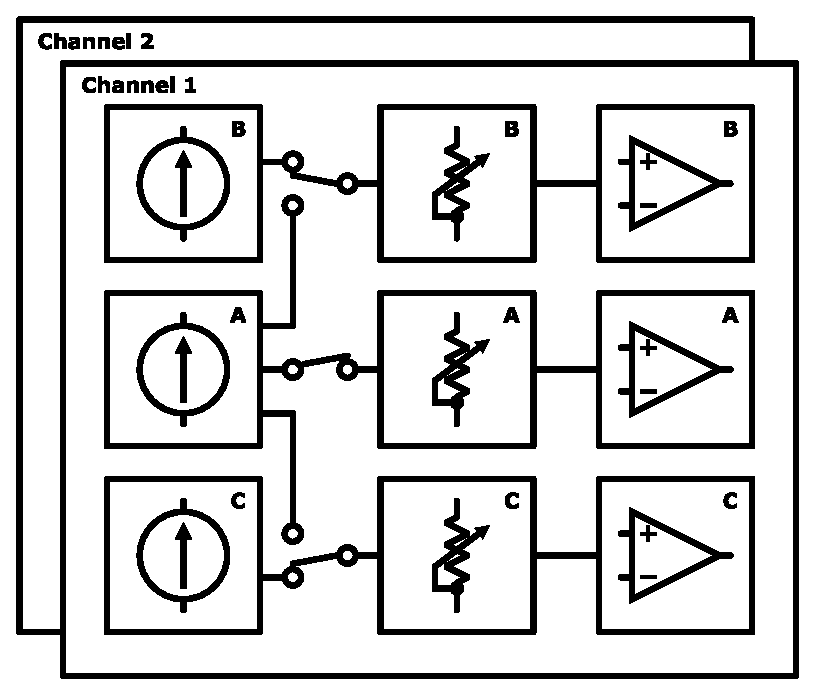
\includegraphics[width=\textwidth]{images/chapter_4/channel/channel_overview.eps}
        \caption{Analog channel block diagram (for more details refer to Appendix \ref{appendix:a}).}
        \label{figure:channel-bd}
    \end{minipage}
\end{figure}

The block diagram shown in Figure \ref{figure:channel-bd} illustrates the organization of the channel, which consists of three sub-channels each with three main blocks: sensor biasing, the \ac{MR} sensor, and signal amplification. The sensor biasing block provides the current required to operate the sensor and converts its output into a voltage signal. The \ac{MR} sensor block is responsible for sensing the magnetic field which is then processed by the signal amplification block. The signal amplification block is the first stage of signal processing and is responsible, as the name implies, for amplifying the weak signal generated by the \ac{MR} sensor, increasing its amplitude to a level that can be reliably processed by the subsequent stages.

The bias circuit A has a topology that allows biasing to three sensor branches. Hence, bias circuit A can be considered the master within its channel as it has the capability to utilize sensors from the other sub-channels (B and C). This feature eases the process of testing and comparing different current source topologies to determine the optimal circuit design for the application. However, it is important to note that an amplification circuit is required for each sensor used.

The size of the \ac{PCB} area required for the channel is directly proportional to the number of channels needed, as each channel comprises three sub-channels. In this interface, illustrated in Figure \ref{figure:channel-pcb}, both channels occupy about 45\% of the \ac{PCB} length. Each sub-channel contains two independent and complex circuits that are connected to the sensor terminals, making it crucial to carefully design and optimize the layout of the \ac{PCB} to minimize cross-talk and interference between sub-channels. This is particularly important for multi-channel systems, where the presence of noise and interference can significantly affect the accuracy and reliability of the measurements.

% ----------------------------------------------------------------------------- Bias Architecture
\subsection{Bias Architecture}

The \ac{SV} sensors are passive elements, thus they need to be biased in order to measure their signals effectively. The biasing architecture, as shown in Figure \ref{figure:bias-full}, is composed of two major circuit blocks: the reference voltage and the biasing topology. While the sensors are shown in the figure for visualization purposes, they will not be discussed in this section. The circuit that supplies the reference voltage is represented at the level of a sub-channel for simplicity, but it will be explained in more detail later in this chapter. The reference voltage provides a stable voltage level that is used as a reference for the biasing topology. The biasing topology, in turn, ensures that the \ac{SV} sensor is operating in its linear range, where its output signal is most sensitive to changes in the input stimulus, as explained in Section \ref{section:soa-mr-sensors}. By carefully controlling the biasing conditions, the \ac{AFE} can achieve accurate and reliable measurements of \ac{SV} sensor signals.

The \ac{SNR} of the system is largely determined by its biasing architecture and the first amplification stage. The biasing noise directly contributes to the overall sensor-referred noise. While the noise from electrical devices that come after the first amplification stage can be attenuated by the stage gain, the achieved noise voltage is still considerably high for the application at hand. Therefore, it is crucial to carefully design the biasing and amplification stages to minimize noise and achieve the best possible \ac{SNR}.

\begin{figure}[!ht]
    \centering
    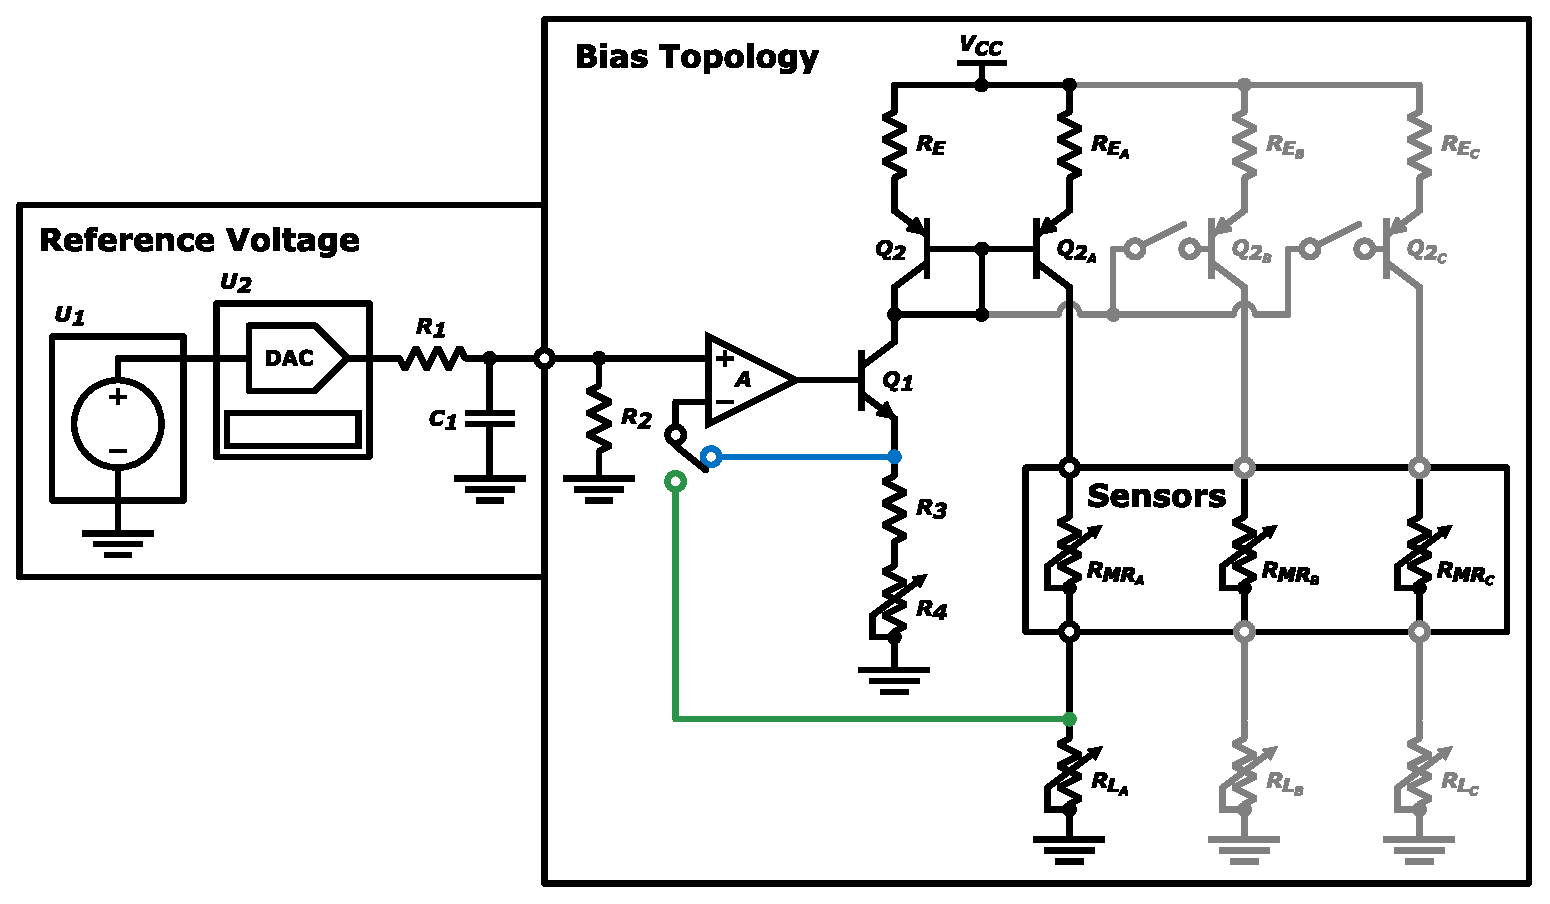
\includegraphics[width=.95\textwidth]{images/chapter_4/channel/bias_full.eps}
    \caption{Biasing architecture (for more details refer to Appendix \ref{appendix:a}).}
    \label{figure:bias-full}
\end{figure}

The bias circuit was designed to encompass two types of topologies, which differ in the position of the sensor relative to the feedback loop. The blue line topology places the sensor outside the feedback loop, and this is the topology that was used in the previous versions of the cytometer and will be emphasized in this thesis. The green line topology places the sensor inside the feedback loop, which is an alternative that has not yet been proven to reduce the noise but is included in the architecture to enable further investigation of this topology without having to modify the \ac{PCB}.

% ............................................................................. Topology with Sensor Outside Feedback Loop
\mytitle{Topology with Sensor Outside Feedback Loop}

\noindent
To obtain a signal from \ac{MR} sensors, a constant current is supplied to the sensors, and the voltage across their terminals is measured. These sensors have a fixed resistance and a variable resistance that changes according to the strength and direction of the magnetic field they are exposed to. By utilizing Ohm's law, the voltage across the sensor's terminals will also change proportionally. By measuring this change in voltage, it is possible to determine the magnitude and direction of the magnetic field being sensed by the sensor (Figure \ref{figure:sv-characteristic}). This section discusses the electronic circuit that was designed by previous studies, mentioned in Chapter \ref{chapter:state-of-the-art}, which produces a constant current output independent of the output load.

The op-amp's high forward gain and differential input design can be utilized to create a nearly perfect \ac{VCCS}, also known as a voltage-to-current converter. To achieve this, the input voltage that needs to be converted (reference voltage) is applied to the non-inverting input terminal of the op-amp $A$, as shown in Figure \ref{figure:bias-openloop}. The inverting input terminal is connected to one end of resistor $R_3$ and the emitter of transistor $Q_1$. The op-amp output ($v_{amp}$) drives the base of the transistor. Due to the high open loop gain of the amplifier, the base of $Q_1$ will be forced to the necessary voltage so that $v_{ref}$ is present across $R_{cur}$. Consequently, the current ($i_{bias}$) in $R_{cur}$ will only flow in the emitter and also appear in the collector of the transistor $Q_1$, and its value is given by:
\begin{equation}
\label{equation:current-value}
    i_{sen} = \frac{v_{ref}}{R_3 + R_4} = \frac{v_{ref}}{R_{cur}} \quad[\mathrm{A}]
\end{equation}
\noindent
In summary, the designed \ac{VCCS} uses an op-amp circuit with a negative feedback loop and a power transistor to produce an output current, which is proportional to the controlled input voltage $v_{ref}$ and the adjustable loop resistor $R_{cur}$ (Equation \ref{equation:current-value}).

After the precision \ac{VCCS}, this current is mirrored using an emitter degenerated current mirror circuit with transistors. A current mirror circuit replicates or mirrors the current flowing through one transistor (the reference transistor) into one or more transistors (the output transistors). The basic idea behind a current mirror circuit is to make the output current independent of the output voltage by using a feedback loop to adjust the current. Adding a resistor in series with the emitter of the transistors increases the stability and linearity of the circuit. This technique is called emitter degeneration. The resistor will reduce the gain of the transistor, but it also makes the circuit less sensitive to variations in the transistor's parameters. In addition, this technique adds a current mirroring factor that depends on the ratio of the emitter resistors. For this application, the goal is to mimic the current generated by the voltage-to-current converter. Therefore, all of the emitter resistors must have the same value, ensuring that $i_{bias} = i_{sen_{\{A, B, C\}}}$. An emitter degenerated current mirror circuit combines these two concepts. In Figure \ref{figure:bias-openloop} circuit, the collector of the reference transistor $Q_2$ is connected to a current source (\ac{VCCS}), and its emitter is degenerated with the $R_E$ resistor. The output transistors $Q_{2_{A}}$, $Q_{2_{B}}$, $Q_{2_{C}}$ are connected in parallel with the reference transistor, and their emitter is also degenerated with a resistor ($R_{E_{A}}$, $R_{E_{B}}$, $R_{E_{C}}$). The base of the output transistors is connected to the base of the reference transistor, forming a feedback loop. This loop ensures that the voltage across the emitter resistors of the two transistors is the same, as long as the degenerated resistors have the same value.

\begin{figure}[!ht]
    \centering
    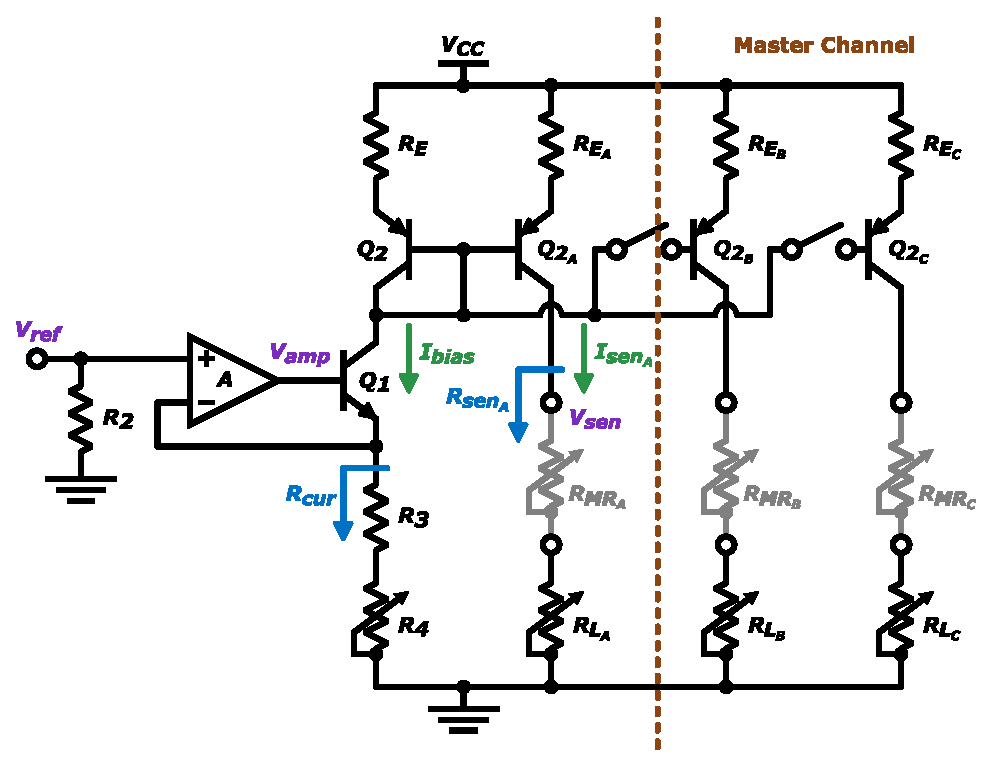
\includegraphics[width=.67\textwidth]{images/chapter_4/channel/bias_openloop.eps}
    \caption{Biasing topology where the sensor is outside the feedback loop (for more details refer to Appendix \ref{appendix:a}).}
    \label{figure:bias-openloop}
\end{figure}

The resistor $R_2$ acts as a pull-down resistor. When the reference voltage $v_{ref}$ is $\mathrm{0~V}$, which comes from a \ac{DAC} as illustrated in Figure \ref{figure:bias-full}, no current flows into the non-inverting input terminal of the op-amp. This can cause the op-amp to saturate and potentially damage the circuit downstream. Therefore, $R_2$ ensures that, in this situation, the non-inverting input is always connected to a low voltage, preventing the op-amp from saturating. Additionally, it is good practice to include an input resistor to account for the op-amp's leakage currents.

Eng. Ricardo Lorena conducted a study in his master's thesis \cite{RicardoL_thesis} where he investigated the bias noise in a circuit using the same topology as the one under discussion. The study focused on the effects of different emitter resistance values on the circuit's noise performance. Through careful experimentation and analysis, he determined that the optimal emitter resistance value was $\mathrm{1~k\Omega}$. This finding was significant because it demonstrated that the choice of emitter resistance can have a notable impact on the circuit's overall noise performance. However, at the time of the practical and theoretical analysis performed in this chapter, Eng. Lorena's work had not yet established the optimal value of the emitter resistance. Therefore, the values of $R_E$, $R_{E_{A}}$, $R_{E_{B}}$, and $R_{E_{C}}$ resistances were all set to the value of $\mathrm{150~\Omega}$ as used in other projects presented in Chapter \ref{chapter:state-of-the-art}. Nevertheless, all noise measurements discussed further in the document were obtained using the optimal value of $\mathrm{1~k\Omega}$, as established by Eng. Lorena's research.

To ensure that the circuit generates the required current for the sensors, it is necessary to ensure that all the transistors must operate in the forward active region. While transistor $Q_2$ always remains in this region, other transistors may not. The reason why transistor $Q_2$ remains forward active is that its base is connected to its collector, resulting in no voltage differential between these, which means that:
\begin{equation}
    \nonumber V_{EC_{Q2}} = V_{EB(on)_{Q2}} \approx 0.7~\mathrm{V} \quad \left(> V_{EC(sat)_{Q2}}\right)
\end{equation}
\noindent
To make sure that the other transistors remain in the forward active region, the designed circuit offers three degrees of freedom that can be adjusted: $v_{ref}$, $R_{cur}$ and $R_{sen}$. By applying the mesh current law to the first branch, which defines the current value, we can determine the operating conditions for transistor $Q_1$.
\vspace{-3mm}
\begin{gather}
    \nonumber -V_{CC} + R_E \cdot i_{sen} + V_{EC_{Q2}} + V_{CE_{Q1}} + v_{ref} = 0 \quad \Leftrightarrow \\
    \nonumber \Leftrightarrow \quad V_{CE_{Q1}} = V_{CC} - R_E \cdot i_{sen} - V_{EC_{Q2}} - v_{ref} \\
    \nonumber \textrm{where} \quad V_{CE_{Q1}} > V_{CE(sat)_{Q1}} \\
    \nonumber \textrm{thus} \quad V_{CE(sat)_{Q1}} < V_{CC} - R_E \cdot i_{sen} - V_{EC_{Q2}} - v_{ref} \quad \Leftrightarrow \\
\label{equation:max-vref}
    \Leftrightarrow \quad v_{ref} < V_{CC} - R_E \cdot i_{sen} - V_{EC_{Q2}} - V_{CE(sat)_{Q1}} \quad [\mathrm{V}]
\end{gather}
\noindent
Equation \ref{equation:max-vref} illustrates the trade-off between $v_{ref}$ and the operation of transistor $Q_1$ in the circuit. If the reference voltage exceeds the value determined by the mesh analysis equation, the transistor will no longer operate in the forward active region. This, in turn, results in the circuit's inability to generate a current that depends on the values of $v_{ref}$ and $R_{cur}$ as intended. The \ac{VCCS} circuit relies on $Q_1$ operating in the forward active region. 

Similarly, the same method can be applied to determine the operating conditions for the transistors $Q_{2_x}$ in the circuit. By analyzing the following mesh equations we can ensure that $Q_{2_x}$ operates in the forward active region and mirrors the generated current for the sensor.
\vspace{-3mm}
\begin{gather}
    \nonumber -V_{CC} + R_{E_x} \cdot i_{sen_{x}} + V_{EC_{Q2_{x}}} + R_{sen_{x}} \cdot i_{sen_{x}} = 0 \quad \Leftrightarrow \\
    \nonumber \Leftrightarrow \quad V_{EC_{Q2_{x}}} = V_{CC} - R_{E_x} \cdot i_{sen_{x}} - R_{sen_{x}} \cdot i_{sen_{x}} \\
    \nonumber \textrm{where} \quad V_{EC_{Q2_{x}}} > V_{EC(sat)_{Q2_{x}}} \\
    \nonumber \textrm{thus} \quad V_{EC(sat)_{Q2_{x}}} < V_{CC} - R_{E_x} \cdot i_{sen_{x}} - R_{sen_{x}} \cdot i_{sen_{x}} \quad \Leftrightarrow \\
\label{equation:max-rsen}
    \Leftrightarrow \quad R_{sen_{x}} < \frac{ V_{CC} - R_{E_x} \cdot i_{sen_{x}} - V_{EC(sat)_{Q2_{x}}} }{ i_{sen_{x}} } \, , \, x \in \{A, B, C\} \quad [\Omega]
\end{gather}
\noindent
Equation \ref{equation:max-rsen} provides a useful guideline for determining the maximum load that the current mirror circuit can support. If the load exceeds this value, the circuit will fail to replicate the required current for the sensors, as the current will not be properly mirrored across the circuit. Therefore, it is important to ensure that the load at the end of the circuit is within the safe operating limits determined by the mesh analysis equation.

It can be observed from Figure \ref{figure:bias-openloop} that this topology can accommodate multiple sensors by adding more current mirror branches. However, only the bias circuit A (shown in Figure \ref{figure:channel-bd}) from each channel can utilize this feature. Although all the bias architecture circuits have the same routing for replication purposes, only the bias circuit A has a physical connection to the sensors from the other circuits B and C, as explained before.

As previously mentioned, \ac{MR} sensors consist of a nominal resistance and a variable resistance that changes with the strength of the magnetic field. The \ac{MR} sensors used in this project were fabricated at \ac{INESC-MN}, and have varying nomimal resistance values. While the initial batches had a nominal resistance of $\mathrm{500~\Omega}$, recent batches have a nominal resistance of $\mathrm{1~k\Omega}$ to $\mathrm{1.5~k\Omega}$. For the sake of simplicity, the following calculations will be performed for a single sensor, and therefore only one output branch will be taken into consideration. Additionally, the emitter resistances for both transistors are set to $\mathrm{150~\Omega}$. The circuit in Figure \ref{figure:bias-openloop} is designed to accommodate different nominal resistance values by adjusting parameters such as $v_{ref}$, $R_{cur}$, and $R_{sen}$. It should be noted that one of the requirements for the architecture is to be able to provide a maximum biasing current of $\mathrm{5~mA}$ for a sensor with a nominal resistance of $\mathrm{500~\Omega}$. Using Equation \ref{equation:max-vref}, one can determine the maximum $v_{ref}$:
\begin{equation}
    \nonumber v_{ref} < 5 - 150 \cdot 5m - 0.7 - 0.4 \quad \Leftrightarrow
    \quad v_{ref} < 3.15~\mathrm{V}
\end{equation}

\noindent
As the reference voltage is provided by a \ac{DAC}, its value can be easily adjusted digitally. To ensure that the transistor $Q_1$ stays in the forward active region, we provide a margin and assume a maximum value of $\mathrm{3~V}$ for $v_{ref}$, which should correspond to the maximum biasing current. By solving Equation \ref{equation:current-value} for $R_{cur}$, we can guarantee that the maximum biasing current is not exceeded.
\begin{equation}
    \nonumber R_{curr} = \frac{3}{5m} = 600~\Omega
\end{equation}

\noindent
As $R_{cur}$ is the sum of a fixed resistance value and a potentiometer that serves the purpose of fine-tuning, the $R_3$ resistance was set to $\mathrm{470~\Omega}$, and the $R_4$ potentiometer was adjusted to match the remaining difference of $\mathrm{130~\Omega}$. With this last tweak, the \ac{VCCS} is now able to provide a $\mathrm{5~mA}$ current. With this adjustment, the \ac{VCCS} can provide a $\mathrm{5~mA}$ current. The final step is to use Equation \ref{equation:max-rsen} to determine the maximum output load that the current mirror can handle, to ensure that it can mimic the biasing current.
\begin{equation}
    \nonumber R_{sen} < \frac{ 5 - 150 \cdot 5m - 0.4 }{ 5m } \quad \Leftrightarrow 
    \quad R_{sen} < 770~\Omega
\end{equation}

$R_{sen}$ is also the sum of two resistances, the sensor and a potentiometer. To simplify the experiment setup and improve measurement accuracy, the sensor was simulated by setting the potentiometer to $\mathrm{500~\Omega}$ and shorting the sensor terminals. In brief, these were the values obtained:
\begin{equation}
    \nonumber v_{ref} = 3~\mathrm{V}\,; \quad R_{cur} = 600~\Omega \,;
    \quad i_{sen} = 5m~\mathrm{A}\,; \quad R_{sen} = 500~\Omega
\end{equation}

Table \ref{tab:pfr-transistors} was obtained by measuring the voltage at terminals of the transistors in the circuit ($Q_1$, $Q_2$, $Q_{2_A}$). These voltage values confirm all the previous calculations to make sure that all the transistors are operating in the forward active region. 

\begin{table}[ht]
    \centering
    \caption{Transistors operating conditions.}
    \begin{small}
    \begin{tabular}[t]{lcc}
    \toprule
    &Voltage [V]\\
    \midrule
    $V_{CE_{Q_1}}$    &   0.594   \\
    $V_{EC_{Q_2}}$    &   0.705  \\
    $V_{EC_{Q_{2_A}}}$ &   1.747   \\
    \bottomrule
\end{tabular}

% \begin{tabular}{|ll|}
% \hline
% \textbf{Transistor} & \textbf{Voltage} \\ \hline
%                     & 0.594            \\ \hline
%                     & 0.705            \\ \hline
%                     & 1.747            \\ \hline
% \end{tabular}
    \end{small}
    \label{tab:pfr-transistors}
\end{table}

\noindent
The transistor $Q_1$ needs to have a voltage $V_{CE}$ greater than the $V_{CE(sat)}$ value, which is $\mathrm{0.4~V}$. In transistor $Q_2$, since its base is connected to its collector, the voltage $V_{EC}$ is equal to the voltage $V_{EB}$, which is approximately $\mathrm{0.7~V}$. The transistor $Q_{2_A}$ has a voltage $V_{EC}$ that corresponds to the difference between the emitter voltage ($5 - 150 \cdot 5m$) and the collector voltage ($500 \cdot 5m$), which is $\mathrm{1.75~V}$. This value must also be greater than $V_{EC(sat)}$.

To more accurately demonstrate the bias topology behavior, the \ac{DAC} responsible for generating the reference voltage was programmed, using an Arduino, to produce a ramp signal ranging from $\mathrm{0~V}$ to $\mathrm{3~V}$, with increments of $\mathrm{0.2~V}$. The measured voltages, which are indicated in purple in Figure \ref{figure:bias-openloop}, were used to generate the following figure, providing a clear representation of the bias behavior.

%\begin{figure}[!ht]
%    \centering
%    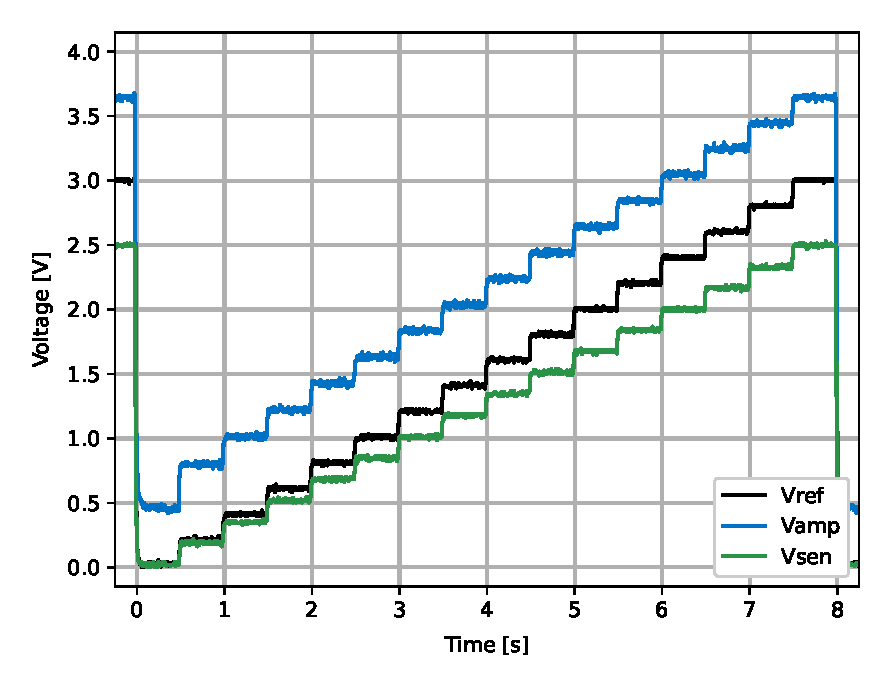
\includegraphics[width=.6\textwidth]{images/chapter_4/channel/bias_exercise.eps}
%    \caption{Biasing exercise.}
%    \label{figure:bias-exercise}
%\end{figure}

\begin{figure}[!ht]
    \centering
    \begin{minipage}{0.45\textwidth}
        \centering
        \includegraphics[clip, trim={9.6cm 2.4cm 16.7cm 14.7cm}, width=.65\textwidth]{images/front_pcb.pdf}
        \caption{3D view of the bias circuit in the PCB.}
        \label{figure:bias-pcb}
    \end{minipage}\hfill
    \begin{minipage}{0.45\textwidth}
        \centering
        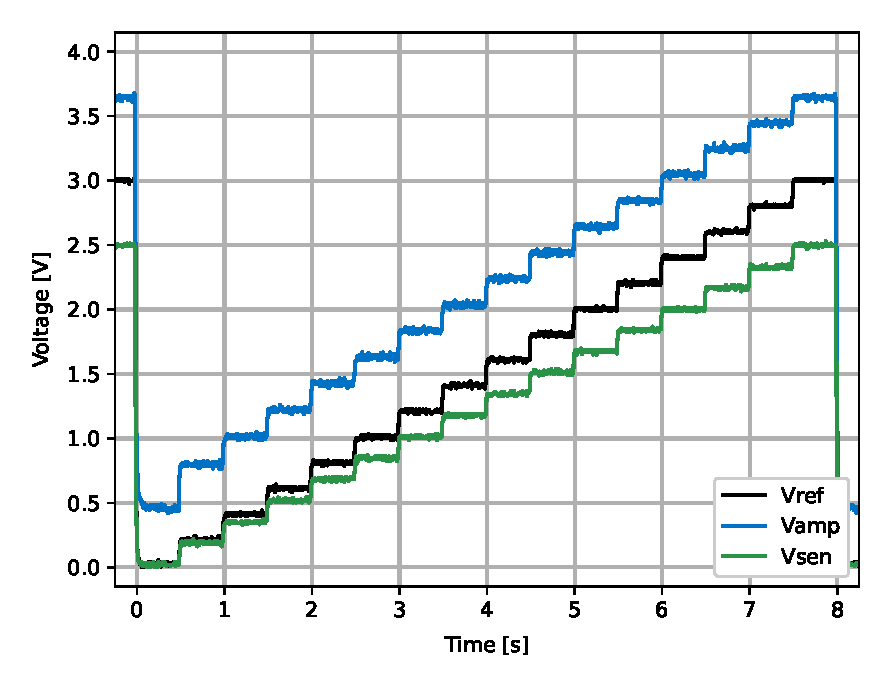
\includegraphics[width=\textwidth]{images/chapter_4/channel/bias_exercise.eps}
        \caption{Biasing exercise.}
    \label{figure:bias-exercise}
    \end{minipage}
\end{figure}

Upon analyzing Figure \ref{figure:bias-exercise}, it is apparent that the topology is performing as intended since the voltage $v_{amp}$ is consistently $V_{CE_{Q1}}$ higher than $v_{ref}$ (as listed in Table \ref{tab:pfr-transistors}). Additionally, the relationship between $v_{ref}$ and $v_{sen}$ can be described by Equation \ref{equation:bias-vsen}, which utilizes Equation \ref{equation:current-value} for simplification. Therefore, $v_{sen}$ is equal to $\nicefrac{5}{6}$ of $v_{ref}$.
\begin{equation}
    v_{sen} = R_{sen} \cdot i_{sen} \quad \Leftrightarrow \quad
    v_{sen} = \frac{R_{sen}}{R_{cur}} \cdot v_{ref} \quad [V]
    \label{equation:bias-vsen}
\end{equation}

The \ac{PCB} layout of this module can be seen in Figure \ref{figure:bias-pcb}. This module encompasses two different topologies, which can be controlled using the visible jumpers (headers or $\mathrm{0~\Omega}$ resistors). The module is housed within an \ac{RFI} shielding to minimize electromagnetic interference caused by external sources or generated within the system itself while ensuring a compact arrangement.
% ............................................................................. Topology with Sensor Outside Feedback Loop

% ............................................................................. Topology with Sensor Inside Feedback Loop
\mytitle{Topology with Sensor Inside Feedback Loop}

\noindent
The work presented in this thesis offers the opportunity to explore an alternative topology where the sensor is placed inside the feedback loop. This topology is included to demonstrate its potential for attenuating noise from all the sources in the biasing topology, except for the noise introduced by the reference voltage, amplifier, and sensor. However, it is worth mentioning that if the sensors have a high capacitance, there is a possibility of amplifier oscillation in this topology. It is important to clarify that the topology involving the sensor inside the feedback loop, developed by Dr. Tiago Costa \cite{6418507}, is referenced in this work to acknowledge its existence and potential advantages. Nevertheless, it is important to note that this topology is not extensively covered or extensively analyzed in detail within the scope of this master's thesis. The primary focus of this thesis is on the previously explained topology, which has been thoroughly examined and optimized. Further investigation and in-depth exploration of the sensor-inside-feedback-loop topology would require dedicated research and analysis beyond the scope of this study.

\begin{figure}[!ht]
    \centering
    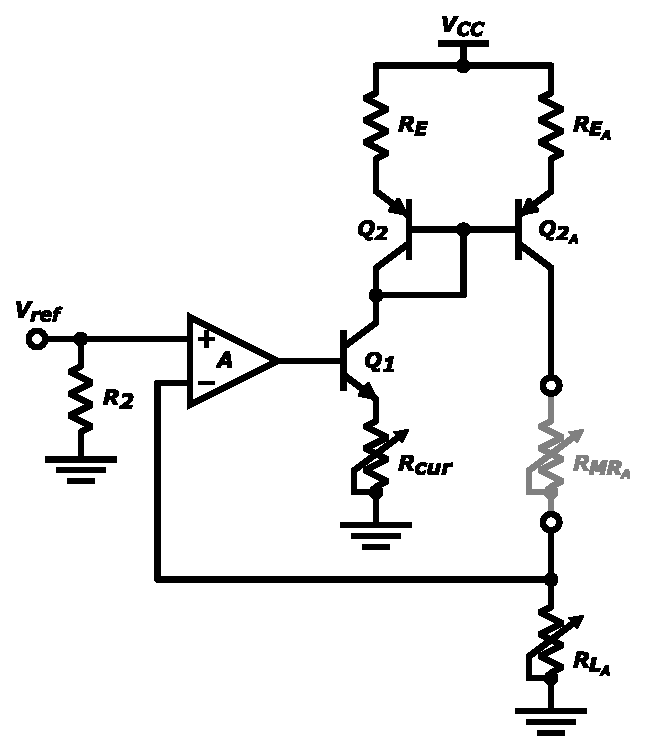
\includegraphics[width=.35\textwidth]{images/chapter_4/channel/bias_closedloop.eps}
    \caption{Biasing topology where the sensor is inside the feedback loop (for more details refer to Appendix \ref{appendix:a}).}
    \label{figure:bias-closedloop}
\end{figure}

\noindent
Figure \ref{figure:bias-closedloop} depicts the sensor-inside-feedback-loop topology, as introduced by Costa \cite{6418507}. In this topology, the voltage reference $v_{ref}$ serves as the input to the amplifier, which generates an output voltage to ensure a desired output current, resulting in a voltage across $R_{L}$ that matches $v_{ref}$. Additionally, transistor $Q_1$ and resistor $R_{cur}$ create an auxiliary current path, enabling the amplifier output to be independent of the sensor resistance value, thereby relaxing the output excursion requirements. It was observed in the study that by choosing $R_{L}$ to be higher than $R_{MR}$, the noise power generated by the current source is attenuated by a factor of $\left(\nicefrac{R_{MR}}{R_{L}}\right)^2$. 
% ............................................................................. Topology with Sensor Inside Feedback Loop

% ............................................................................. Reference Voltage
\mytitle{Reference Voltage}

\noindent
To ensure that the biasing circuit performs correctly, it requires a precise and stable reference voltage. However, using the power supply to generate the reference voltage is often not ideal due to the inherent noise and fluctuations that can arise in the supply voltage. To overcome this issue, a common approach is to use a voltage reference generator paired with a \ac{DAC} to generate and precisely adjust the reference voltage.

This circuitry to generate a reference voltage is a widely used technique in electronic circuits, particularly in applications where a stable and accurate current source is required, such as in industrial automation, instrumentation, and control systems. By using a \ac{DAC}, the reference voltage can be adjusted digitally, providing precise control over the output current of the biasing circuit. In the work of Germano \textit{et al.} \cite{Germano2006MICROSYSTEMFB}, this technique was implemented to generate a reference voltage in the biochip platform, as discussed in Chapter \ref{chapter:state-of-the-art}. By utilizing the generator and a \ac{DAC}, they were able to achieve a stable and accurate current source, even in the presence of environmental factors such as temperature variations and power supply fluctuations. Additionally, this approach provides high flexibility as arbitrary waveforms can be generated by programming the \ac{DAC}.

The reference voltage schematic used in the \ac{AFE} interface is depicted in Figure \ref{figure:vref-schematic}. While the biasing topology can provide a bias current regardless of the load, variations in the sensor's nominal resistance may occur. However, by using a \ac{DAC} to individually adjust each current that feeds the sensors, this resistance difference can be overcome without the need for more accurate components such as precise resistors or potentiometers. In addition, calibration can be performed via software, eliminating the need for manual adjustments to the \ac{PCB}. As a result, the user can simply select the values in the application, making the process more efficient and less prone to errors.

\begin{figure}[!ht]
    \centering
    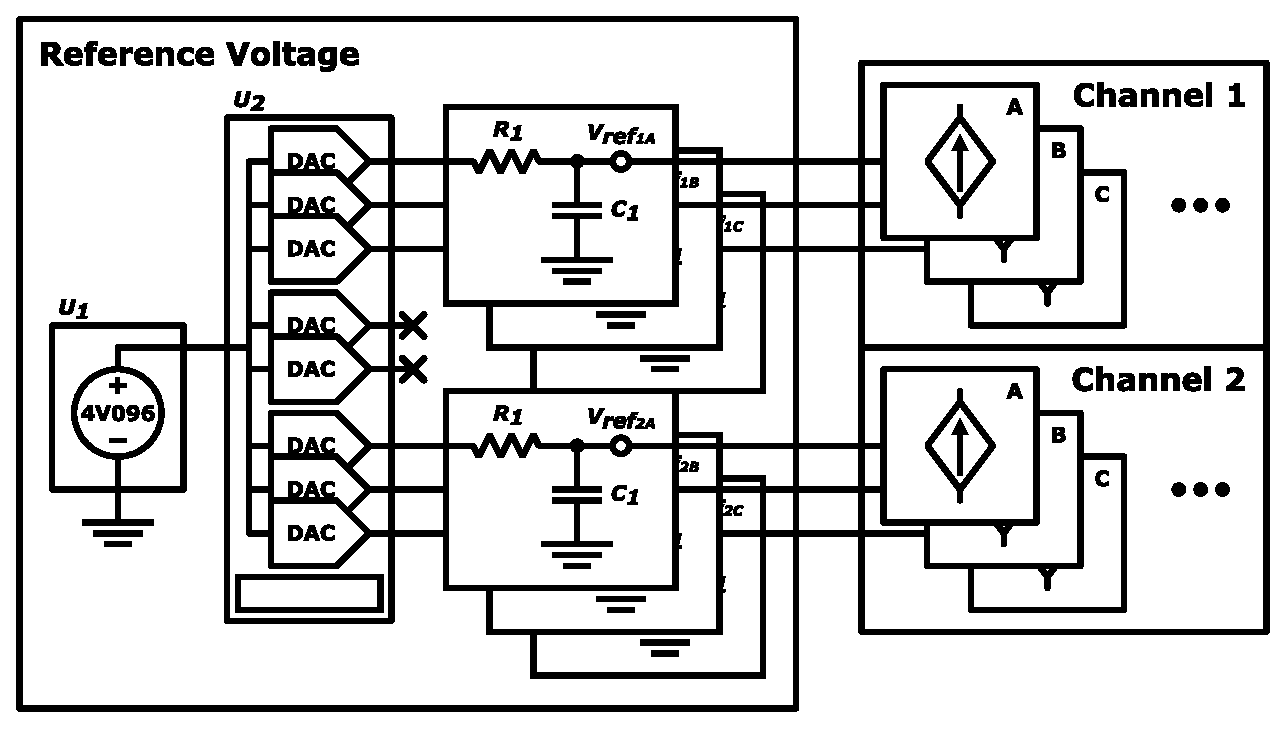
\includegraphics[width=.8\textwidth]{images/chapter_4/channel/vref.eps}
    \caption{Reference voltage schematic (for more details refer to Appendix \ref{appendix:a}).}
    \label{figure:vref-schematic}
\end{figure}

To accommodate the six different sub-channels on the board, a \ac{DAC} with a minimum of six channels is required, as shown in Figure \ref{figure:channel-bd} where there are two main channels each with three sub-channels. In addition, it is important to use an external input voltage for the \ac{DAC}, as an ultra-low noise reference voltage is required to minimize the impact of noise on the output signal of the sensors. Figure \ref{figure:vref-schematic} illustrates how this is achieved through the use of $U_1$ and $U_2$, where $U_1$ provides the input voltage to the \ac{DAC} $U_2$, which then adjusts each output voltage based on its programming. As for the voltage reference, it must meet two requirements: have low-noise characteristics and provide a voltage higher than $\mathrm{3~V}$ to enable a $\mathrm{5~mA}$ biasing current to flow through the sensor when its nominal resistance is $\mathrm{500~\Omega}$, as previously determined. Before each \ac{DAC} outputs feeds the bias circuit, some additional filtering is performed using a \ac{RC} filter, acting as a \ac{LPF}. The \ac{RC} circuit will smooth the output waveform of the \ac{DAC}, by filtering out high-frequency noise components and harmonics present in the signal, leaving only the low-frequency signal intact. The cutoff frequency of the \ac{RC} filter depends on the values of $R$ (resistance) and $C$ (capacitance) used in the circuit -- and can be calculated using the following Equation \ref{equation:cutoff-frequency}.
\begin{equation}
    f_c = \frac{1}{2\pi RC} \quad [\mathrm{Hz}]
    \label{equation:cutoff-frequency}
\end{equation}

The selection criteria for the \ac{DAC} \ac{IC} was straightforward. Analog Devices has a product family called \textit{nano}DAC+ that includes several compact package \ac{IC}s with low-power, rail-to-rail strings of \ac{DAC}s whose outputs have high precision. This family of \ac{IC}s is great because it gives flexibility in terms of the communication protocol to control the \ac{IC}. For the schematic shown in Figure \ref{figure:vref-schematic}, $U_2$ belongs to the $\mathrm{AD567xx}$ family, which was the best choice in terms of versatility. Depending on the \ac{IC}, the communication protocol can be either \ac{SPI} or \ac{I2C}, the input voltage can be either internal or external, and the resolution can be either 16-bit or 12-bit. For this project, the $\mathrm{AD5676}$ was used because it encompasses \ac{SPI}, external input voltage, and 16-bit resolution. Furthermore, by selecting a versatile family like the \textit{nano}DAC+, there is no need to limit the pool search according to the communication protocol for future \ac{IC}s in other circuits.

The reference used in the design is the $\mathrm{ADR444}$, also from Analog Devices, it uses an XFET reference, providing better noise performance than buried Zener references, which was the type used in the previous work (Chapter \ref{section:soa-interfaces}). Additionally, the output voltage of $\mathrm{4.096~V}$, making it ideal to be controlled with a minimum of a 12-bit \ac{DAC} for achieving a resolution of $\mathrm{1~mV}$. The \ac{RC} filter, comprised of $R_1$ ($\mathrm{100~\Omega}$) and $C_1$ ($\mathrm{100~\mu F}$), has a cutoff frequency of approximately $\mathrm{16~Hz}$, calculated using Equation \ref{equation:cutoff-frequency}. The main purpose of the filter is to provide a clean \ac{DC} current to the sensors, free from switching noise introduced by the \ac{DAC}s, clock harmonics, and high-frequency noise components. The capacitance value of $C_1$ is the highest available in a 0603 package, which is $\mathrm{100~\mu F}$, while the resistance value was chosen based on the settling time of the filter output. A lower cutoff frequency leads to a longer settling time. This circuit has been thoroughly tested, as shown in a previous figure (Figure \ref{figure:bias-exercise}).

Even though the reference voltage and the biasing topology were designed to provide a \ac{DC} current to the sensors, further studies using an \ac{AC} current can be performed by removing the \ac{RC} filter. Biasing in \ac{AC} is a common practice \cite{8526523, PMID24761029, TIM.2013.2296417}, and allows for the output signal from the sensors to be shifted into a higher frequency where the noise is lower, thus improving the \ac{SNR}. However, it is important to note that this work focuses on \ac{DC} biasing.

\begin{figure}[!ht]
    \centering
    \includegraphics[clip, trim={0.1cm 1.7cm 22.9cm 14.7cm}, width=.5\textwidth]{images/front_pcb.pdf}
    \caption{3D view of the reference voltage circuit in the PCB.}
    \label{figure:vref-pcb}
\end{figure}

Figure \ref{figure:vref-pcb} showcases the reference voltage module integrated into the cytometer platform. This module introduces a new feature, and to ensure adaptability in the event of malfunction, the headers are responsible for providing access to all circuit inputs, outputs, and power supplies. If a failure were to occur, potentially compromising the entire board, a separate small \ac{PCB} can be affixed to the headers, providing a fixed solution for the problem. This arrangement allows for the isolation and disconnection of the faulty circuit from the rest of the board while utilizing the small \ac{PCB}. Moreover, the headers also offer control capabilities specific to this circuit.
% ............................................................................. Reference Voltage
% ----------------------------------------------------------------------------- Bias Architecture

% ----------------------------------------------------------------------------- Amplification Scheme
\subsection{Amplification Scheme}

As explained in Section \ref{section:mfc-principle}, when a magnetic particle passes through a magnetic sensor and is excited by a permanent magnet, the magnetic sensor reacts to the field generated between the magnet and the particle, resulting in the generation of a pulse. The purpose of this application is to measure the number of pulses per sample, which corresponds to the number of analytes present in the sample. The resulting data will be analyzed by a computer and undergo digital processing. In order to convert the sensor signal, we will be using \ac{ADC}s. It's important to take the quantization resolution into consideration, especially since the sensor response signal typically falls in the hundreds of $\mathrm{\mu V}$ range, which is close to the first decision level of most \ac{ADC}s. To make sure that we utilize the maximum dynamic range of the \ac{ADC} and reduce the quantization noise associated with the conversion, we need to amplify the signal.

The amplification scheme used in this work is based on Eng. Ruben Afonso work in Section \ref{section:soa-interfaces}, which was developed from Tiago Costa's thesis \cite{TiagoC_thesis}. In ultra-low noise applications, differential amplifiers are commonly used to increase the \ac{SNR} ratio and minimize the impact of external interference on measurement accuracy. These amplifiers work by taking the difference between two input voltages while suppressing any voltage that is common to both inputs. By doing so, they can reduce the impact of common noise between the positive and negative terminals.

The amplification scheme used in this work is illustrated in Figure \ref{figure:amp-schematic}, and it employs the $\mathrm{AD8429}$ instrumentation amplifier ($U_1$) from Analog Devices. This \ac{IC} is an excellent choice for measuring extremely small signals, thanks to its high-precision architecture. The $\mathrm{AD8429}$ features a high-bandwidth and a high-gain architecture that can be adjusted from $\mathrm{1~V/V}$ to $\mathrm{10000~V/V}$. However, it's important to note that the voltage input offset will also be amplified, accordingly to the gain. Therefore, when choosing the gain for the amplifier, a trade-off must be made between the differential amplifier's dynamic response and the voltage input offset.

\begin{figure}[!ht]
    \centering
    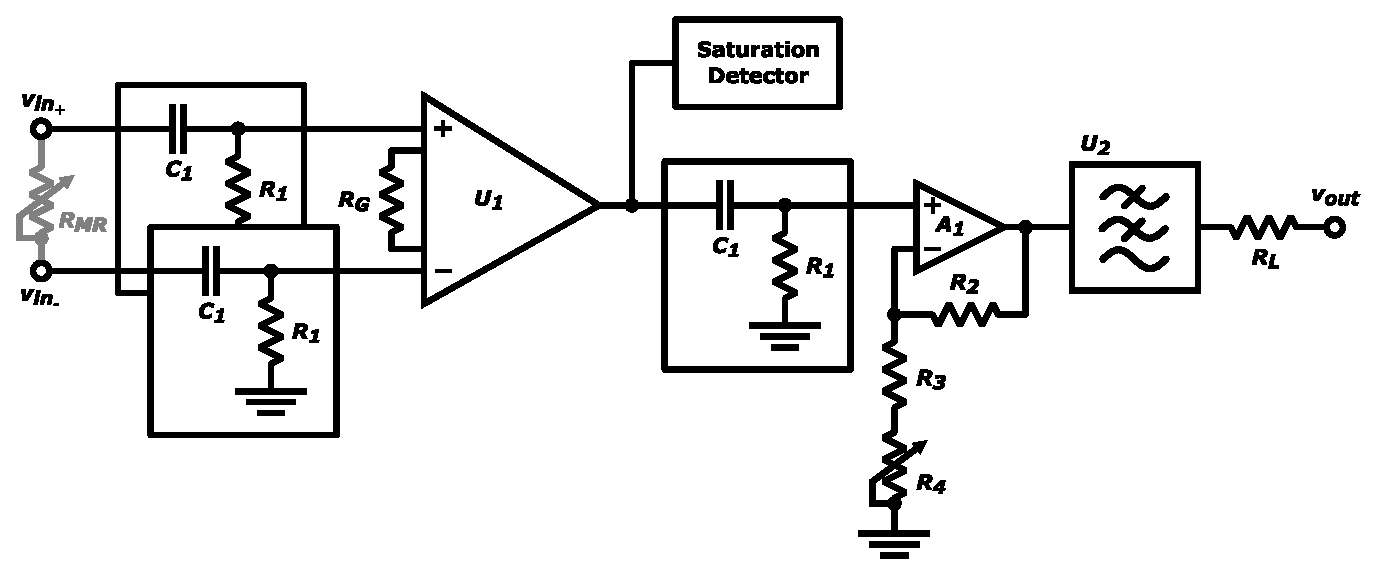
\includegraphics[width=.65\textwidth]{images/chapter_4/channel/amp.eps}
    \caption{Amplification and filtering schematic (for more details refer to Appendix \ref{appendix:a}).}
    \label{figure:amp-schematic}
\end{figure}

In applications developed at \ac{INESC} that utilize \ac{SV} sensors, the required bandwidth is typically low \cite{1.3562915, s90604119}. However, the necessary bandwidth can vary depending on factors such as the size of the particles or the sensor design. To ensure accurate flow rate measurements up to $\mathrm{30~\mu l/min}$, a bandwidth of at least $\mathrm{100~kHz}$ is required, according to a recent study by Dr. Diogo Caetano \cite{DiogoC_thesis}. The signal response frequency is directly proportional to the velocity of the particles flowing through the sensors. To process the signals from the sensors, it is crucial to select an amplifier with a dynamic response that can respond to the signal without causing excessive attenuation. However, increasing the amplifier gain reduces the available bandwidth. This relationship is given by the \ac{GBWP}, which represents the maximum gain that can be achieved for a given bandwidth. For the $\mathrm{AD8429}$ instrumentation amplifier, the \ac{GBWP} is $\mathrm{15~MHz}$. Therefore, if the gain is set to $\mathrm{1000~V/V}$, the dynamic response of the amplifier is reduced to $\mathrm{150~kHz}$. This response is sufficient to provide satisfactory performance when processing the sensors' signals, while still leaving room for any potential flow rate increases. This gain is also sufficient to prevent the signal from undershooting or overshooting when the amplified input noise is added to the sensor's signal. If the amplified noise adds too much voltage to the signal, it may exceed the amplifier rails, leading to the clipping of the output signal. This is undesirable as it can cause distortion of the signal and compromise the accuracy of the measurement.

Even though amplifying the signal by a factor of 1000 is significant, it is not enough to fully utilize the dynamic range of the \ac{ADC}. As a result, the amplification circuit in Figure \ref{figure:amp-schematic} combines the instrumentation amplifier with a non-inverting amplifier, creating a cascade or multistage amplifier architecture. This extra amplifier helps to improve the overall gain, allowing for better utilization of the \ac{ADC} dynamic range. It is known that adding an extra amplifier will not significantly impact the overall noise of the system. This is due to the Friss formula, which states that when several devices are cascaded, the total noise figure is given by:
\begin{equation}
     F = F_{A_1} + \frac{F_{A_2} - 1}{G_1} + \frac{F_{A_3} - 1}{G_1 G_2} + ... + \frac{F_{A_n} - 1}{G_1 G_2\,...\,G_{n-1}}  \quad \mathrm{\left[\frac{dB}{Hz}\right]}
    \label{equation:friss-formula}
\end{equation}

\noindent
Where $F$ is the noise figure of the n-th stage and $G_n$ is the power gain of the n-th stage. With Equation \ref{equation:friss-formula}, it becomes clear that the $F$ of the initial stage in an amplification chain has the most significant effect on the total noise figure than the following stages. This is because the $F$ of each stage is divided by the gain of all the previous stages. This means that the circuits from the input signal to the first amplification stage play a crucial role in determining the overall noise of the \ac{AFE} system, and can be considered to be the key circuits for establishing the system \ac{SNR}.

The gain of the non-inverting amplifier ($A_1$) is given by Equation \ref{equation:non-inverting-gain}. In this circuit, the resistances $R_2$, $R_3$, and $R_4$ were adjusted so that the gain of the second-stage amplifier is $\mathrm{10~V/V}$, which gives an overall amplification gain of $\mathrm{10000~V/V}$. This high gain is necessary to boost the signal from the hundreds of microvolts to the volts range, which is required for proper signal acquisition and processing. As such, $R_2$ is a $\mathrm{9.1~k\Omega}$ and the sum of $R_3$ and $R_4$ is approximately $\mathrm{1~k\Omega}$. The adjustable $R_4$ allows more precision over the gain, which otherwise wasn't possible, using only two resistances.

\begin{equation}
     G_{A_2} = 1 + \frac{R_2}{R_3 + R_4}
    \label{equation:non-inverting-gain}
\end{equation}

The amplification process not only boosts the desired signal but also amplifies any unwanted noise or interference that may be present. Thus, it is essential to remove any unwanted noise from the signal before processing it further. To achieve this, each stage of the multi-stage amplification scheme is equipped with an \ac{RC} filter, which acts as a \ac{HPF}. These \ac{RC} filters are represented inside the squares in Figure \ref{figure:amp-schematic}. The signal response from the sensors includes a \ac{DC} component inherent to the bias, as well as an \ac{AC} component that carries the magnetic information \cite{DiogoC_thesis}. To remove the \ac{DC} component, which is not relevant, and the low-frequency noise generated in the biasing topology, one \ac{HPF} filter is used at both inputs of the differential amplifier. The \ac{RC} filter at the output of the differential amplifier, removes the voltage offset and reduces the amplification noise introduced in that stage. The filters used in both amplification stages have an identical cutoff frequency because they use capacitors $C_1$ and resistors $R_1$ with the same value. The cutoff frequency is approximately $\mathrm{160~Hz}$, which is calculated using Equation \ref{equation:cutoff-frequency}, as $C_1$ is $\mathrm{100~nF}$ and $R_1$ is $\mathrm{10~k\Omega}$.

In Figure \ref{figure:amp-schematic}, the final component ($U_2$) is a 4\textsuperscript{th}-order \ac{LPF} filter, implemented using the $\mathrm{LTC1563\textnormal{-}2}$ \ac{IC}. The filter has a sharper roll-off, providing improved frequency selectivity and more effectively attenuating frequencies outside the passband. A key advantage of the $\mathrm{LTC1563\textnormal{-}2}$ \ac{IC} is that its cutoff frequency can be easily adjusted using a single resistor value, making it a flexible component that can be tailored to specific needs. It's important to note that the cutoff frequency must be chosen carefully to avoid aliasing. According to the Nyquist theorem, the minimum sampling rate should be at least twice the highest frequency component of the input signal. In this case, the maximum signal frequency is assumed to be $\mathrm{100~kHz}$, so the minimum sampling rate must be $\mathrm{200~kSPS}$. Without the filter, the amplification scheme would require an \ac{ADC} with at least $\mathrm{300~kSPS}$, since the differential amplifier's band-width is $\mathrm{150~kHz}$. By setting the $U_2$ filter's cutoff frequency to approximately $\mathrm{100~kHz}$, the requirements for choosing the \ac{ADC} are lower. In summary, this filter serves as an anti-aliasing filter, effectively removing any high-frequency components of the signal that may cause aliasing, while still allowing the system to accurately capture relevant frequency components. The inclusion of the $R_L$ resistor at the end of the filter is vital for the proper operation of the circuit. According to the datasheet, the output of the \ac{IC} is designed to drive signals around $\mathrm{\pm~5~V}$ when connected to a load greater than $\mathrm{1.2~k\Omega}$. By adding a resistor with a value of $\mathrm{1.2~k\Omega}$ as the load, the output signal is ensured to fall within the required range. This load resistor restricts the output current of the filter, allowing it to function within the specified parameters, especially when connected to a low-impedance acquisition device.

To analyze the behavior of the amplification and filtering scheme, the transfer function of the system is plotted in Figure \ref{figure:amp-bode}. The experiment was performed using an Analog Discovery\footnote{Analog Discovery 2 system document can be found \href{https://digilent.com/reference/test-and-measurement/analog-discovery-2/start}{here}.} to sweep through frequencies and an attenuator to prevent signal saturation in the first stage of amplification. This experiment was conducted at each step of the amplification chain: instrumental amplifier (1\textsuperscript{st} Stage); non-inverting amplifier (2\textsuperscript{nd} Stage); and output (\ac{LPF} Filter).

%\begin{figure}[!ht]
%    \centering
%    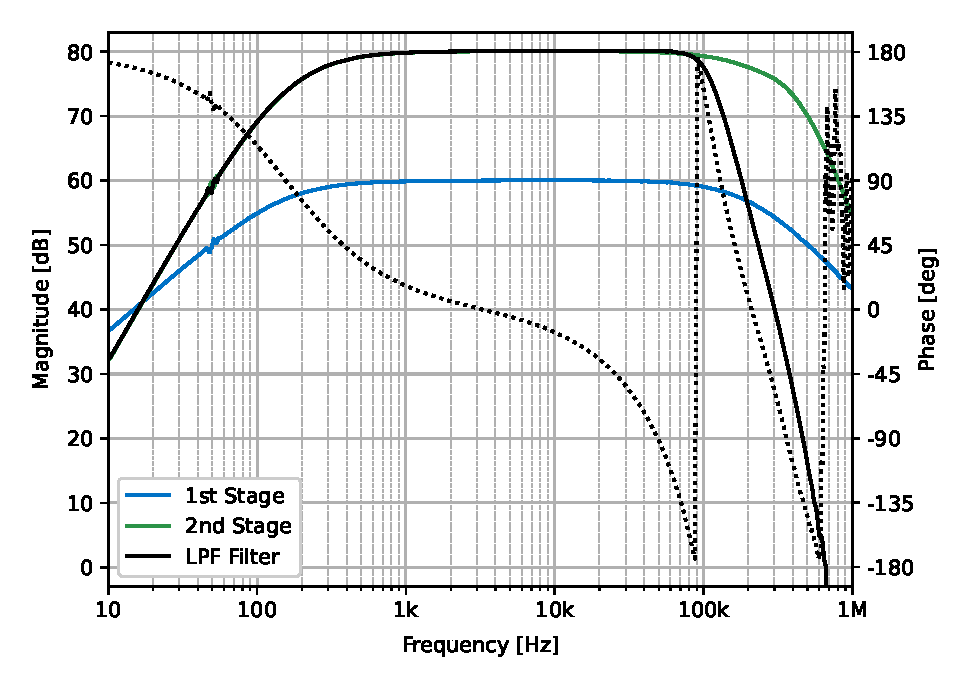
\includegraphics[width=.55\textwidth]{images/chapter_4/channel/amp_bode_v2.eps}
%    \caption{Amplification scheme bode diagram.}
%    \label{figure:amp-bode}
%\end{figure}

\begin{figure}[!ht]
    \centering
    \begin{minipage}{0.45\textwidth}
        \centering
        \includegraphics[clip, trim={9.6cm 11cm 16.7cm 6.2cm}, width=.65\textwidth]{images/front_pcb.pdf}
        \caption{3D view of the amplification scheme circuit in the PCB.}
        \label{figure:amp-pcb}
    \end{minipage}\hfill
    \begin{minipage}{0.45\textwidth}
        \centering
        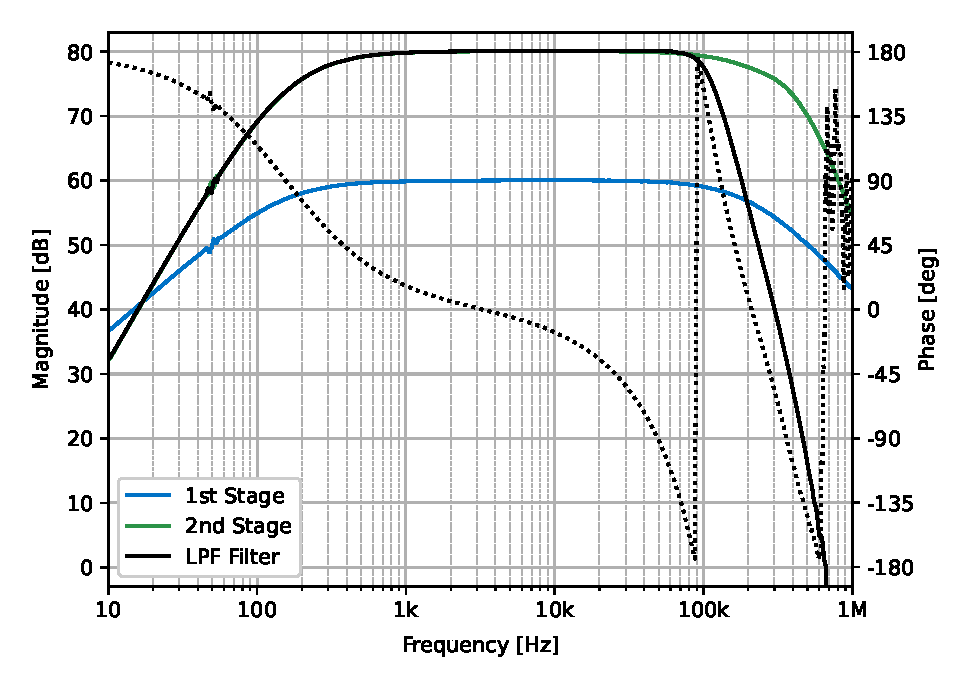
\includegraphics[width=\textwidth]{images/chapter_4/channel/amp_bode_v2.eps}
        \caption{Amplification scheme bode diagram.}
        \label{figure:amp-bode}
    \end{minipage}
\end{figure}

As mentioned before, Figure \ref{figure:amp-bode} shows the transfer function of the amplification circuit. The blue trace represents the output of the instrumentation amplifier. It is expected a $\mathrm{20~dB/dec}$ increase per decade due to the presence of a \ac{HPF} \ac{RC} input filter in the instrumentation amplifier. The gain starts to decrease as the frequency approaches $\mathrm{150~kHz}$, accordingly to the \ac{GBWP}. The voltage gain in the baseline is also in agreement with the gain defined by $R_G$, which is $\mathrm{1000~V/V}$.
\begin{equation}
     \nonumber G_{U_1} = 20\cdot \log{10}\,(1000) = 60~\mathrm{dB}
\end{equation}

\noindent
The green and black traces represent the output of the non-inverting amplifier and the filter output, respectively. With the addition of another filter to the $A_1$ amplifier input, which is also an \ac{HPF} \ac{RC} filter, a $\mathrm{40~dB/dec}$ decrease is expected. In contrast, the black trace at $\mathrm{100~kHz}$ shows an $\mathrm{80~dB/dec}$ decrease compared to the green trace due to the 4\textsuperscript{th} order \ac{LPF} filter. The total system gain ($\mathrm{10000~V/V}$) also matches the gain depicted in Figure \ref{figure:amp-bode}.
\begin{equation}
     \nonumber G_{total} = 20\cdot \log{10}\,(1000 \cdot 10) = 80~\mathrm{dB}
\end{equation}

Figure \ref{figure:amp-pcb} depicts the \ac{3D} representation of the amplification schematic. This circuit bears resemblance to the one used in the previous version of the cytometer, but with improved debugging capabilities. Notably, each stage of the circuit now features a coaxial switch at its output, enabling the disconnection of the circuit at that specific point. This functionality proves highly valuable for noise measurements and overall circuit debugging purposes. To minimize electromagnetic interference from external sources or within the system, the module is securely enclosed within a shielding specifically designed for \ac{RFI}.

% ............................................................................. Saturation Detector
\mytitle{Saturation Detector}

\noindent
The useful information present in the signal response of the sensors is \ac{AC}, which is why there are \ac{HPF} at the input of the differential amplifier to remove any \ac{DC} components. However, during amplification by the first stage in the signal chain, the inherent noise of the amplification process is added to the signal. Furthermore, due to the very high gain of the differential amplifier, the system is highly sensitive to environmental interference. As a result, the output signal of the first stage can be prone to saturation, when the signal exceeds the output levels that the amplifier can provide. In either case, the amplifier's output becomes a \ac{DC} signal with a voltage value of either $V_{DD}$ or $V_{EE}$, depending on the scenario. If a signal becomes saturated and proceeds to the next stage, it will encounter another \ac{HPF}, which can cause the complete removal of the signal -- since saturation removes the \ac{AC} component, while the filter removes the \ac{DC} component. This can be misleading to the user, who is not aware of what has occurred and could assume that everything is functioning correctly, even though the signal has been lost. To alert for this and avoid negative consequences, this will approach the circuit that has been developed to tackle this issue. 

Figure \ref{figure:sat} shows the circuit for the "Saturation Detector" block in Figure \ref{figure:amp-schematic}. The circuit can be divided into three segments: Comparator, Delay, and Shift. The previous cytometer interface only had the comparator segment, which was only capable of alerting the user when the differential amplifier was constantly saturating. This was due to the fact that saturation can occur in very short time intervals, making it difficult for the human eye to perceive the \ac{LED} turning on. To address this issue, the delay segment was developed to keep the \ac{LED} on for a period of time that is perceivable to the human eye. In addition, the shift block was also created to allow the signal to be used in digital processing.

\begin{figure}[!ht]
    \centering
    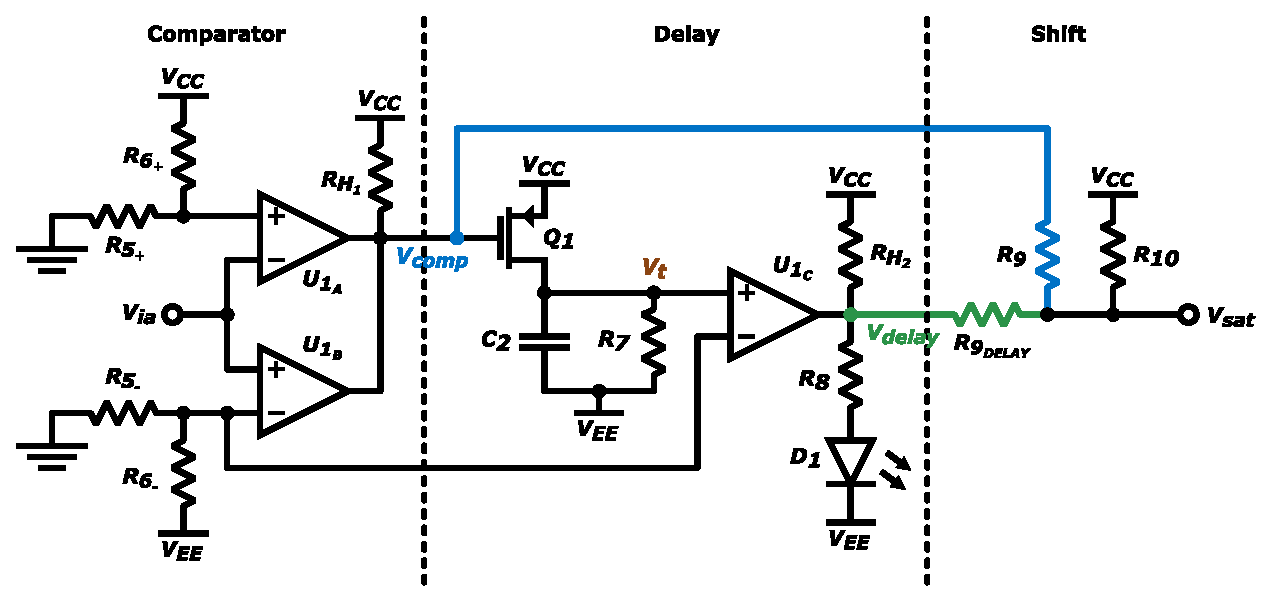
\includegraphics[width=.85\textwidth]{images/chapter_4/channel/sat.eps}
    \caption{Saturation detector circuit (for more details refer to Appendix \ref{appendix:a}).}
    \label{figure:sat}
\end{figure}

The saturation block takes the output of the instrumentation amplifier ($v_{ia}$) as input to identify unreliable signals. One of the comparator terminals is connected to a voltage reference set by the voltage divider $R_5$ and $R_6$, and the other is connected to the input voltage being compared $v_{ia}$. When the input voltage is higher than the reference voltage, the output of the comparator saturates to the negative supply voltage, indicating a low output state. Conversely, when the input voltage is lower than the reference voltage, the output of the comparator saturates to the positive supply voltage, indicating a high output state. There are two comparators, one for each rail of the amplifier. In summary, the behavior of the comparator segment can be defined by Equation \ref{equation:sat-comparator}.
\begin{equation}
    v_{comp} =
    \begin{cases}
      V_{EE}&, \, v_{ia} > \frac{R_{5_+}}{R_{5_+}+R_{6_+}} \cdot V_{CC}\\
      V_{CC}&, \, \frac{R_{5_-}}{R_{5_-}+R_{6_-}} \cdot V_{EE} < v_{ia} < \frac{R_{5_+}}{R_{5_+}+R_{6_+}} \cdot V_{CC}\\
      V_{EE}&, \, v_{ia} < \frac{R_{5_-}}{R_{5_-}+R_{6_-}} \cdot V_{EE}
    \end{cases}
    \quad [\mathrm{V}]
    \label{equation:sat-comparator}
\end{equation}

\noindent
The main objective of this complementary circuit is to minimize its size while fulfilling its purpose. Therefore, the choice of the comparator was based on the number of comparators present in the \ac{IC}. As shown in Figure \ref{figure:sat}, this circuit requires three comparators: two for the comparator segment and one for the delay segment. The $\mathrm{LM2901}$ was selected because it has four comparators and requires the same supply voltage as the other \ac{IC}s used in this circuit. The $\mathrm{LM2901}$ output consists of an open-collector transistor, which requires a pull-up resistor to drive the output. Thus, a pull-up resistor ($R_{H_1}$) was placed in the output of $U_{1_A}$ and $U_{1_B}$. For the reference voltage, $R_5$ and $R_6$ resistors were set to $\mathrm{10~k\Omega}$ and $\mathrm{11~k\Omega}$, respectively, resulting in a voltage of $\mathrm{\pm2.38~V}$ fed into the comparator. The specific voltage polarity depends on the purpose of the comparator. This reference voltage was chosen because the input signal ($v_{ia}$) is typically in the hundreds of $\mathrm{mV}$ range (at that amplification stage), so the reference voltage is significantly different from the signal values, allowing for efficient saturation detection.

In the delay segment, the purpose is to, as the name implies, delay the period where the signal is saturating and provide some visual feedback of the saturation happening to the user, via a \ac{LED}. This delay feature can be achieved using a capacitor that charges rapidly when the output of the comparators goes low, and slowly discharges when it goes back to the high default state. However, to make this possible, a switch is required that only charges the capacitor when the $v_{comp}$ signal goes to $V_{EE}$. A P-channel transistor ($Q_1$) can be used as a switch, with the $v_{comp}$ signal connected to the gate and $V_{CC}$ connected to the source. When $V_{SG} > V_{TH}$, the switch "closes," and the voltage at the source appears on the drain, allowing the capacitor to charge almost instantly, as $R_{on}$ of the transistor is really low. The output of the delay segment comparator is determined by the voltage divider formed by $R_{H_2}$ and $R_8$, only when the positive input of the comparator ($v_t$) is greater. This leads to an anode voltage higher than the cathode of $D_1$, turning the \ac{LED} on. In contrast, when the negative input is greater, the output is pulled down to $V_{EE}$, and the \ac{LED} remains off since no current flows through it. When $v_{comp}$ is no longer in low-state, the switch $Q_1$ turns off and the capacitor starts discharging through resistor $R_7$.
\begin{equation}
    v_{delay} =
    \begin{cases}
        V_{CC} \cdot \frac{R_{8}}{R_{8}+R_{H_2}} + V_{EE} \cdot \frac{R_{H_2}}{R_{8}+R_{H_2}}&, \, v_{U_{1_C}+} > v_{U_{1_C}-} \\
        V_{EE}&, \, v_{U_{1_C}+} < v_{U_{1_C}-}
    \end{cases}
    \quad [\mathrm{V}]
    \label{equation:sat-delay}
\end{equation}

\noindent
Equation \ref{equation:sat-delay} summarizes the output states of $U_{1_C}$, which were obtained by applying the superposition theorem to the comparator's high-state output voltage and despising the diode resistance. It is noteworthy that when $R_8$, the resistor that limits the current to $D_1$, and $R_{H_2}$ have equal resistance values, the high-state output voltage is $\mathrm{0~V}$. Therefore, $v_{delay}$ is $\mathrm{-5~V}$ when $v_{ia}$ is not saturated, and $\mathrm{0~V}$ when it is. The duration for which the \ac{LED}s stay on is determined by multiple factors, including the charging time of the capacitor ($t_{charge}$), the duration of signal saturation ($t_{sat}$), and the discharge time of the capacitor ($t_{discharge}$). These factors collectively influence the total duration of \ac{LED} activation, as shown by Equation \ref{equation:led-on}.
\begin{equation}
    t_{LED_{on}} = t_{charge} + t_{sat} + t_{discharge} \quad [\mathrm{s}]
    \label{equation:led-on}
\end{equation}

The charging time of the capacitor can be considered negligible, as it occurs almost instantaneously, as explained earlier. The duration of signal saturation can vary, but the discharge time of the capacitor remains constant and can be adjusted to achieve a longer duration for the \ac{LED} to stay on ($t_{LED_{on}}$). By modifying the discharge time, the desired duration of \ac{LED} activation can be extended. To increase the duration of the \ac{LED} illumination, the negative reference voltage of the comparator segment is used. This enables $U_{1_C}$ to stay high, for a longer period of the capacitor discharge time and a correspondingly longer on-time for the \ac{LED}.
\begin{equation}
    t_{discharge} = R_7C_2 \cdot\ln {\left(\frac{V_{CC} - V_{EE}}{\frac{R_{5_-}}{R_{5_-}+R_{6_-}} \cdot V_{EE} - {V_{EE}}}\right)} \quad [\mathrm{s}]
    \label{equation:led-off}
\end{equation}

\noindent
Equation \ref{equation:led-off} provides the time required for the capacitor to discharge based on the values of resistor $R_7$ and capacitor $C_2$. This equation was derived by solving the differential equation that describes the voltage across the capacitor as a function of time, and then applying it to the specific voltages in the circuit. By analyzing the equation, one can determine the relationship between the discharge time and the values of $R_7$ and $C_2$. Adjusting these component values allows for controlling the duration of \ac{LED} activation.

%\begin{figure}[!ht]
%    \centering
%    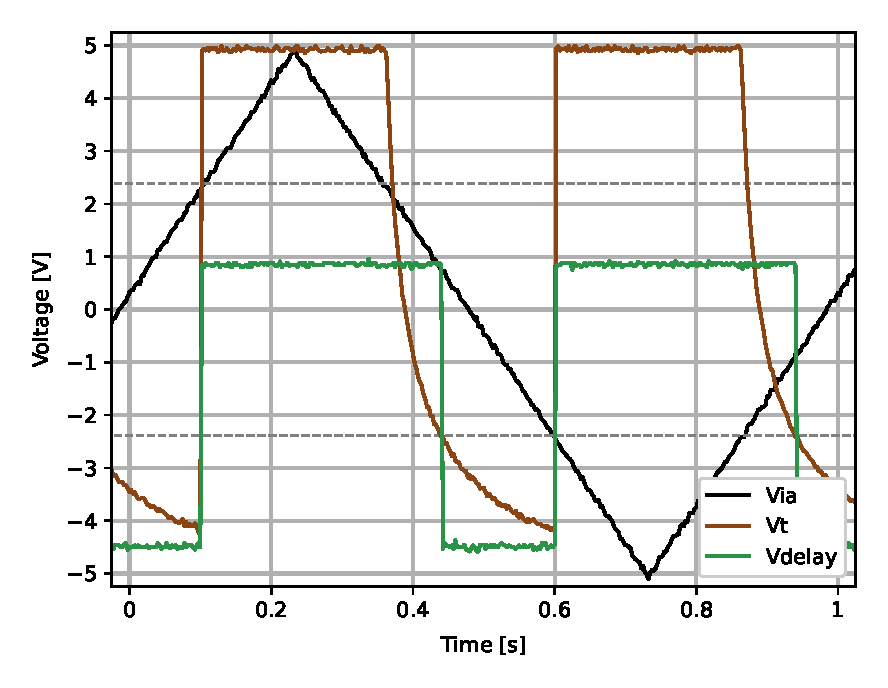
\includegraphics[width=.5\textwidth]{images/chapter_4/channel/sat_ex.eps}
%    \caption{Saturation detector functional test.}
%    \label{figure:sat-ex}
%\end{figure}

\begin{figure}[!ht]
    \centering
    \begin{minipage}{0.45\textwidth}
        \centering
        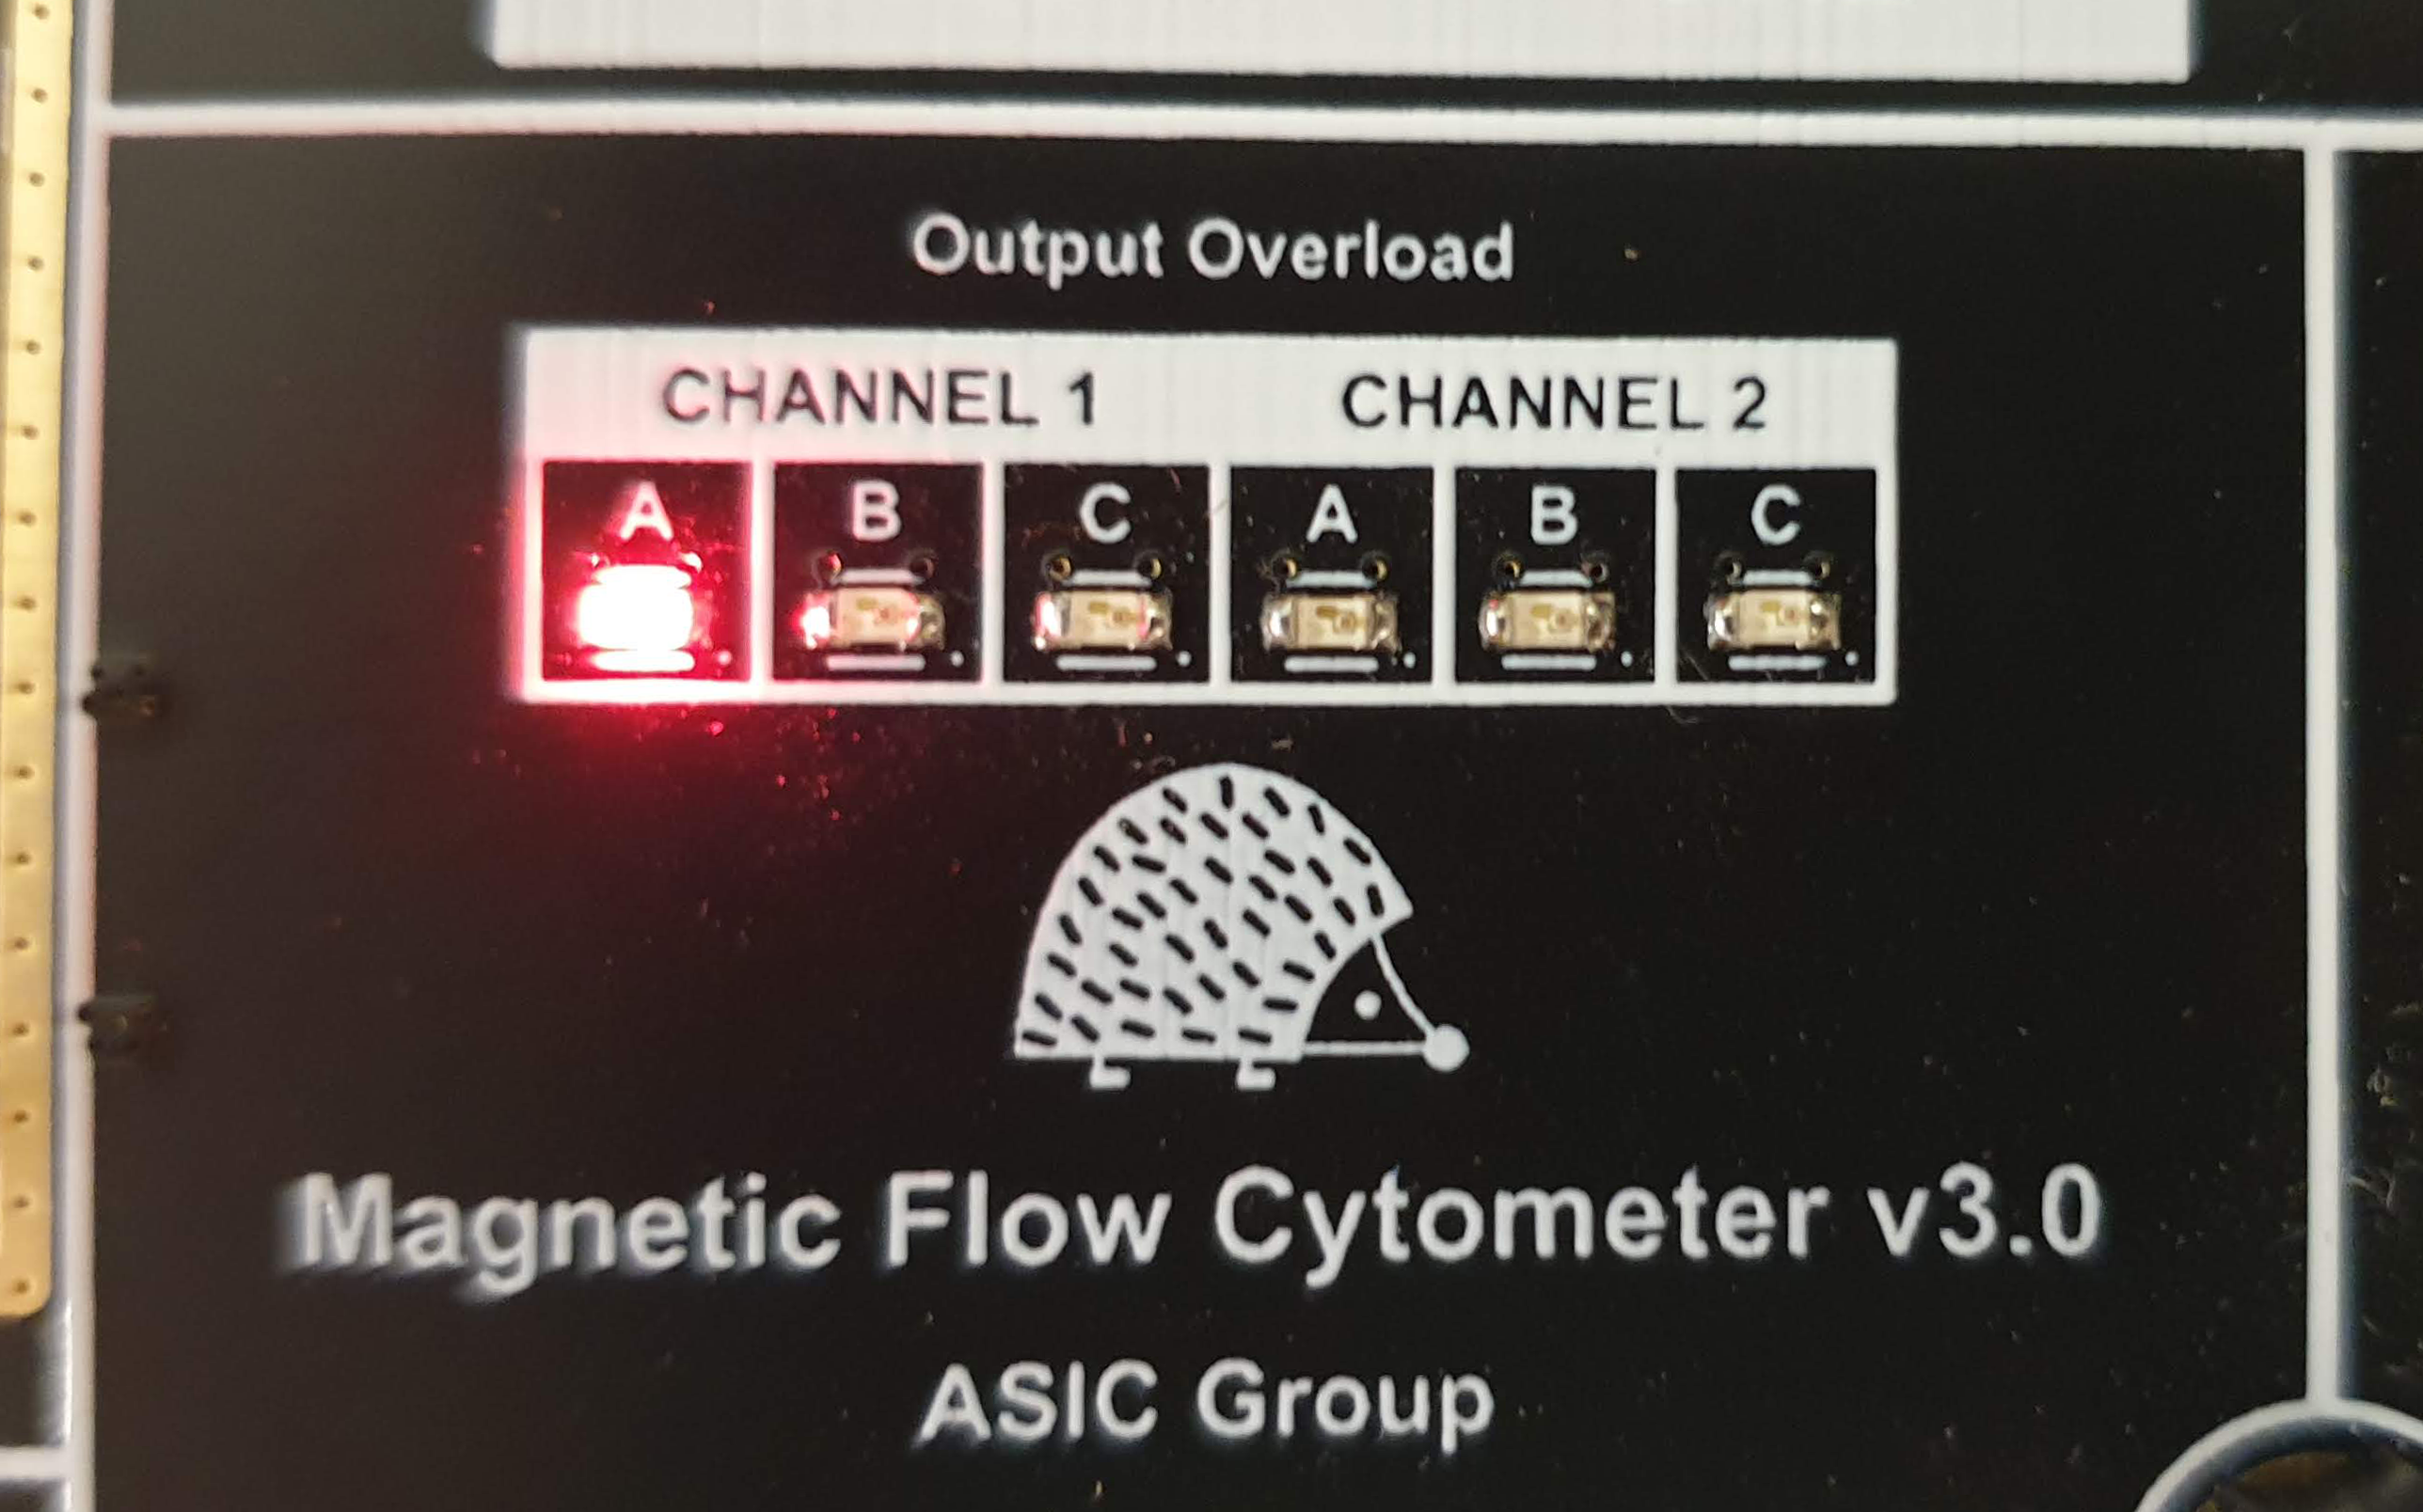
\includegraphics[width=\textwidth]{images/chapter_4/channel/sat_leds.png}
        \caption{Saturation detector LED display with channel 1-A saturating.}
        \label{figure:sat-leds}
    \end{minipage}\hfill
    \begin{minipage}{0.45\textwidth}
        \centering
        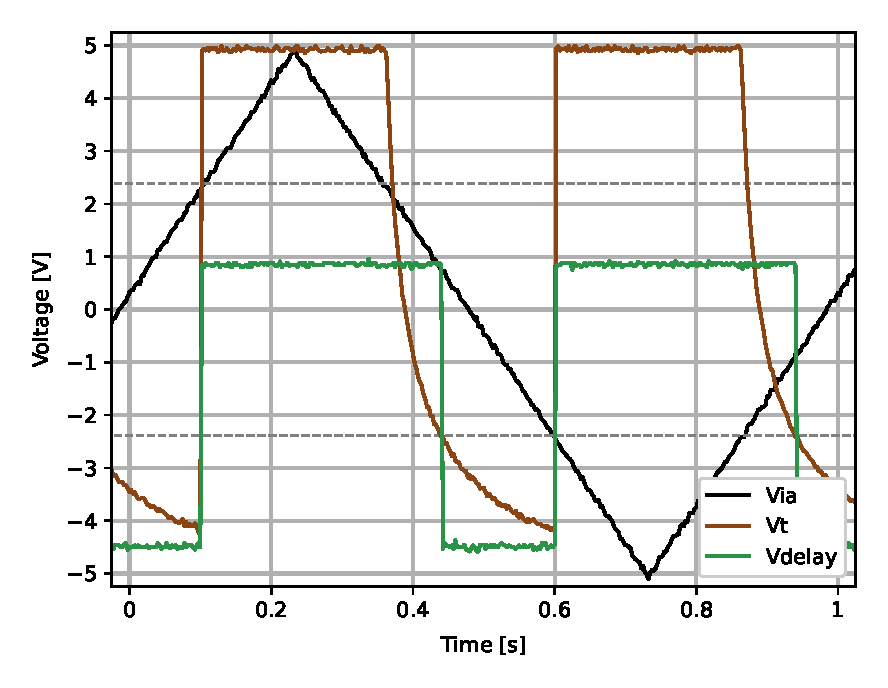
\includegraphics[width=\textwidth]{images/chapter_4/channel/sat_ex.eps}
        \caption{Saturation detector functional test.}
        \label{figure:sat-ex}
    \end{minipage}
\end{figure}

Figure \ref{figure:sat-ex} illustrates the functionality of the delay segment designed to increase the duration of the illuminated state of the \ac{LED}. The trace names and colors correspond to the voltages shown in Figure \ref{figure:sat}. From the graph, it is evident that the signal $v_{ia}$ remains in a saturated state for approximately $\mathrm{0.25~ms}$ ($t_{sat}$). The grey dashed lines represent the positive and negative reference voltage levels, which are set at $\mathrm{\pm 2.38~V}$. When the black trace is above these reference levels, it indicates saturation. The signal $v_{delay}$ extends the high state beyond the saturation period, as explained earlier. This is achieved through the manipulation of the capacitor discharge time, which increases the signal duration by approximately $\mathrm{60~ms}$, independently of the saturation time. To achieve this, the resistor $R_7$ was set to $\mathrm{20~k\Omega}$, and the capacitor $C_2$ was chosen to be $\mathrm{10~\mu F}$, according to Equation \ref{equation:led-off}. The graph demonstrates the effectiveness of this segment in prolonging the illuminated state of the \ac{LED}, displayed in Figure \ref{figure:sat-leds}. Additionally, it is worth noting that the $v_{delay}$ signal does not actually range from $\mathrm{-5~V}$ to $\mathrm{0~V}$ as initially expected. This deviation is attributed to the presence of the forward voltage drop ($V_{on}$) across the diode $D_1$, which introduces a small offset in the signal.

The last segment of the circuit is the "Shift", which is responsible for changing the range of the signal to make it suitable for digital processing. This is achieved through a voltage divider formed by one of the $R_9$ resistors and $R_{10}$. It is important to note that for the $v_{sat}$ signal to operate correctly, only one of the $R_9$ resistors should be present in the circuit, either $R_9$ or $R_{9_{delay}}$. If both resistors are used simultaneously, it can lead to erroneous results due to conflicting signals. In order to obtain accurate digital measurements, it is recommended to use the signal originating from $v_{comp}$, which has not undergone any delay. This signal should be used as the reference for determining when the input signal is saturated. It is worth noting that the delayed signal should only be used for visual feedback purposes and not for digital processing. This is because the delayed signal has undergone a significant delay and does not accurately represent the input signal. The following equation represents the $v_{sat}$ output signal, concerning $v_{comp}$ signal.
\begin{equation}
    v_{sat} = v_{comp} \cdot \frac{R_{10}}{R_{9}+R_{10}} + V_{CC} \cdot \frac{R_{9}}{R_{9}+R_{10}} \quad [\mathrm{V}]
    \label{equation:sat-vsat}
\end{equation}

\noindent
Equation \ref{equation:sat-vsat} describes the output voltage, $v_{sat}$, of the saturation detector circuit in terms of the resistors $R_9$ and $R_{10}$ and the signal $v_{comp}$. However, if these two resistors have equal values, $v_{sat}$ can be simplified to either $V_{CC}$ or $\mathrm{0~V}$, depending on the state of $v_{comp}$. Specifically, when the circuit's output is low, the differential amplifier is saturating, and $v_{sat}$ is $\mathrm{0~V}$. Conversely, when $v_{sat}$ is high, the differential amplifier is functioning correctly and there are no errors in the results.

\begin{figure}[!ht]
    \centering
    \includegraphics[clip, trim={15.2cm 3cm 11.7cm 14.3cm}, width=.25\textwidth]{images/back_pcb.pdf}
    \caption{3D view of the saturation detector circuit in the PCB.}
    \label{figure:sat-pcb}
\end{figure}

Figure \ref{figure:sat-pcb} shows the saturation module integrated into the \ac{PCB}. This module has been meticulously designed to maintain a small and compact form factor without compromising the overall functionality of the platform. Its primary function is to identify potential errors within the acquired samples, which couldn't be detected at stages beyond the first amplification stage. Hence, the circuit has been positioned behind the amplification scheme, effectively utilizing space on the bottom layer without compromising the routing on the top layer while serving its intended purpose.

% ............................................................................. Saturation Detector
% ----------------------------------------------------------------------------- Amplification Scheme
% ############################################################################# Channel

% ############################################################################# Sensor Addressing
\section{Sensor Addressing}
\label{chapter:fe-addressing}

The chip, housing the highly sensitive \ac{MR} sensors essential for this application, has been designed and manufactured at \ac{INESC-MN}. The chip comprises a total of 28 sensors, arranged across 8 microfluidic channels, ensuring optimal coverage. To facilitate seamless integration with different chip batches, the chip is wire-bonded to a \ac{PCB} developed by Eng. Ruben Afonso. This custom-designed \ac{PCB}, an integral part of the cytometer platform, plays a crucial role in providing stable electrical connections and mounting support for the chip. A key objective of the sensor addressing module is to simplify the process of acquiring signals from the 28 individual sensors housed within the chip. To achieve this, the module circuit incorporates digitally controlled multiplexers as a gateway between the sensor \ac{PCB} and the \ac{AFE}. The sensor addressing module not only optimizes the functionality of the cytometer platform but also offers the flexibility to adapt to various experimental requirements.

%\begin{figure}[!ht]
%    \centering
%    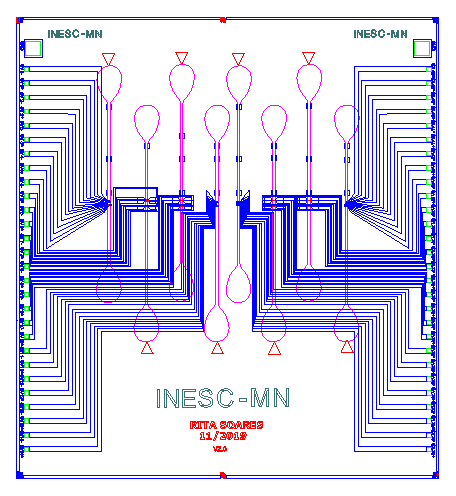
\includegraphics[width=.35\textwidth]{images/chapter_4/sensor_addressing/sensor_chip.eps}
%    \caption{Sensor chip fabricated at INESC-MN.}
%    \label{figure:sensor-chip}
%\end{figure}

In the previous cytometer platform, the sensor selection process involved soldering $\mathrm{0~\Omega}$ resistors to act as switches. This platform has only 2 analog channels, so the resistors on the top layer controlled one channel, while the resistors on the bottom layer controlled the other. Additionally, there were only 7 resistors available on each side of the board, limiting the selection to only one column of the sensor's \ac{PCB} on each side. As a result, users had to physically orientate the board to access different columns, which posed a constraint. As this application requires multidisciplinary work, the previous method required researchers to have soldering skills and knowledge of interpreting schematics to change the sensor. The reliance on manual soldering and technical understanding added an additional layer of complexity and potential challenges for users operating the cytometer platform. To address these limitations and enhance user convenience, the sensor addressing module has been designed and implemented.

The circuit design for the sensor addressing module is simple and efficient. It utilizes 6 multiplexers, with each multiplexer dedicated to one analog channel on the board. To meet the requirements outlined in the previous chapter, each multiplexer should be capable of switching between at least 3 sensors. Most multiplexer \ac{IC}s have a number of inputs that are multiple of two. This allows to effectively switch between four sensors using just one \ac{IC} without increasing the circuit space in the board. Since the amplification is performed differently and the sensors are arranged as a differential pair, the \ac{IC} must have a minimum of 8 inputs to accommodate the multiplexing of 4 sensors. Regarding internal configuration, the switches inside the \ac{IC} can be arranged as a 2x4:1 or an 8:8 structure. In addition to the appropriate configurations, it is crucial to select a multiplexer \ac{IC} with a low on-resistance for the switches. This ensures that the resistance value of the sensors is minimally impacted by the multiplexer circuitry, thereby maintaining accurate and reliable measurements. Regarding the supply voltage for the \ac{IC}, it is important to consider the biasing topology and the output characteristics of the sensors. In this case, as the sensor is referenced to the ground, the sensor's output voltage never goes below zero. As a result, the supply voltage for the multiplexer \ac{IC} can be either single or double.

\begin{table}[ht]
    \centering
    \caption{Multiplexer ICs for the sensor addressing circuit.}
    \begin{small}
    \begin{tabular}{ccccccccc}
\toprule
\multirow{2}{*}{IC} & \multirow{2}{*}{Ron $\mathrm{[\Omega]}$} & \multicolumn{2}{c}{Configuration} & \multicolumn{2}{c}{Supply $\mathrm{[V]}$} & \multicolumn{3}{c}{Comm. Protocol} \\
\cmidrule(r){3-4} \cmidrule(r){5-6} \cmidrule(r){7-9}
                    &                                 & 4:1             & 8:8             & Single        & Double ($\pm$)           & I2C       & SPI       & Bits       \\
\midrule
ADG1609             & 4.5                             & x               &                 & 3.3 -- 16      & 3.3 --  8    &           &           & x          \\
MAX4639             & 3                               & x               &                 & 1.8 -- 5       &  2.5        &           &           & x          \\
ADG739              & 2.5                             & x               &                 & 2.7 -- 5.5     &                  &           & x         &            \\
ADG71(4/5)          & 2.5                             &                 & x               & 2.7 -- 5.5     & 2.5        & x         & x         &            \\
ADGS1414D           & 1.5                             &                 & x               & 12             & 5 -- 15     &           & x         &            \\
MAX14662            & 0.5                            &                 & x               & 1.6 -- 5.5     & 5.5        & x         & x         & x          \\
\bottomrule 
\end{tabular}
    \end{small}
    \label{tab:sensor-ics}
\end{table}

Table \ref{tab:sensor-ics} presents the various candidate multiplexer \ac{IC}s considered for integration into the circuit. Upon reviewing the table, the $\mathrm{MAX14662}$ \ac{IC} emerged as the most suitable choice due to its versatile configuration options and communication protocol compatibility. Furthermore, it exhibited the lowest on-resistance ($R_{on}$) among the options listed. However, despite its favorable characteristics, the $\mathrm{MAX14662}$ \ac{IC} presented a drawback in terms of noise introduction. The level of noise generated by this \ac{IC} was deemed high, rendering it impractical for use in the circuit. The $\mathrm{ADGS1414D}$ also emerged as an interesting choice for integration into the circuit. This \ac{IC} is particularly appealing due to its design catering to large system channel density. Notably, the $\mathrm{ADGS1414D}$ offers the advantage of route-through pins for digital signals and power supplies. This feature significantly simplifies the routing process, especially when using a 4-layered \ac{PCB}. Unfortunately, the $\mathrm{ADGS1414D}$ price was found to be extremely high, making it economically unviable for the intended application. Furthermore, it is worth mentioning that two other potential options, the $\mathrm{ADG714}$ and $\mathrm{ADG739}$ multiplexer \ac{IC}s, were unfortunately out of stock at the time of design. These \ac{IC}s were considered due to their compatibility with the communication protocol used in the reference voltage circuit. After considering the available options, the final decision was made between $\mathrm{ADG1609}$ and $\mathrm{MAX4639}$. The $\mathrm{ADG1609}$ was ultimately selected due to its greater diversity in terms of supply voltage options. This feature enables further studies and experimentations in the biasing topology, particularly for scenarios that may require a wider supply range.

In order to provide each channel with access to every sensor within the chip, a switch matrix circuit would be required. However, the implementation of such a circuit, with a large number of rows and columns, poses significant challenges in terms of routing in discrete electronics. Additionally, the approach used in the previous platform, employing $\mathrm{0~\Omega}$ resistors as switches, would not be feasible for the current system, as the number of channels has tripled. Considering these factors, the most suitable solution was to utilize several multiplexer \ac{IC}s. This allows each analog channel to select between 4 \ac{SV} sensors.

\begin{table}[ht]
    \centering
    \caption{Addressable sensors per analog channel.}
    \begin{small}
    \begin{tabular}{cccccc}
\toprule
\multicolumn{2}{c}{Channel} & \multicolumn{4}{c}{MR Sensors} \\
\midrule
\multirow{3}{*}{1}    & A   & 1     & 8      & 15    & 22    \\
                      & B   & 2     & 9      & 16    & 23    \\
                      & C   & 3     & 10     & 17    & 24    \\
\midrule
\multirow{3}{*}{2}    & A   & 4     & 11     & 18    & 25    \\
                      & B   & 5     & 12     & 19    & 26    \\
                      & C   & 6     & 13     & 20    & 27    \\
\bottomrule
\end{tabular}
    \end{small}
    \label{tab:sensor-per-channel}
\end{table}

Table \ref{tab:sensor-per-channel} displays the allocation of sensors for each analog channel within the system. It is evident from the table that out of the total 28 sensors available, only 24 can be utilized. Unfortunately, sensors number 7, 14, 21, and 28 are not accessible through any of the analog channels. This limitation should be acknowledged as a drawback that the chip design team at \ac{INESC-MN} must take into account when designing future batches of chips.

\begin{figure}[!ht]
    \centering
    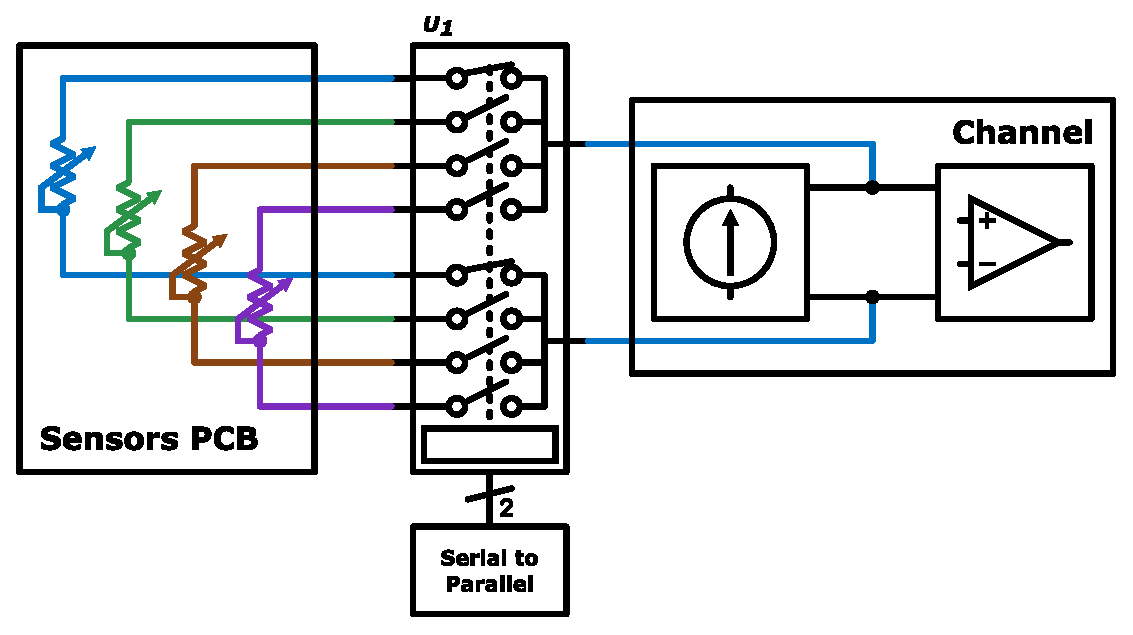
\includegraphics[width=.7\textwidth]{images/chapter_4/sensor_addressing/sensormux.eps}
    \caption{Sensor addressing module (for more details refer to Appendix \ref{appendix:a}).}
    \label{figure:sensormux}
\end{figure}

Figure \ref{figure:sensormux} provides an illustration of the schematic diagram of the \ac{IC} used in the module and demonstrates how it integrates into the cytometer system. As depicted, the first inputs of either outputs are selected, indicated by the closed switch. This results in the blue sensor being routed to the output of the multiplexer, which then connects to the output of the biasing topology and the input of the amplification scheme. The previous sections of the document have elaborated on these circuits, which encompass a sub-channel. While the figure only displays four sensors on the sensor \ac{PCB} for simplicity, it is important to note that the actual \ac{PCB} houses a total of 28 sensors. Each multiplexer within the module is responsible for assigning a specific sensor to one of the six sub-channels present in the two main channels. The purpose of the serial to parallel block shown in Figure \ref{figure:sensormux} will be further discussed in the document.

Figure \ref{figure:sensormux-ex} serves as evidence of the circuit's successful operation. The diagram was generated by utilizing an Arduino to control both the voltage reference and the addressing of the sensor circuits. The objective of this graph is to validate the module's functionality by measuring the voltage drop at the output terminals of the biasing topology, with $v_{sen}$ corresponding to the voltage depicted in Figure \ref{figure:bias-openloop}. To accentuate the changes and highlight the circuit's performance, a sensor \ac{PCB} was employed. However, instead of the chip typically present on the \ac{PCB}, resistors with values well within the capabilities of the biasing circuit were utilized. This allowed for a clearer demonstration of the desired modifications. For the purpose of this test, the voltage reference was meticulously controlled to provide a fixed reference voltage, thereby ensuring a consistent current flow through the multiplexer terminals. The current was precisely set at $\mathrm{1~mA}$ by adjusting the value of $R_{sen}$ in the biasing topology. As the sensor load resistor $R_{L}$ held no relevance for this specific test scenario, it was adjusted to $\mathrm{0~\Omega}$. The resistors used to simulate the sensors in this setup had specific resistance values assigned to them, namely $\mathrm{500~\Omega}$, $\mathrm{1~k\Omega}$, $\mathrm{1.5~k\Omega}$, and $\mathrm{2~k\Omega}$. According to Ohm's law, these resistance values correspond to voltage values of $\mathrm{0.5~V}$, $\mathrm{1~V}$, $\mathrm{1.5~V}$, and $\mathrm{2~V}$ respectively at the $v_{sen}$ node. This test validates the functionality of the module and demonstrates its effectiveness in controlling sensor addressing.

%\begin{figure}[!ht]
%    \centering
%    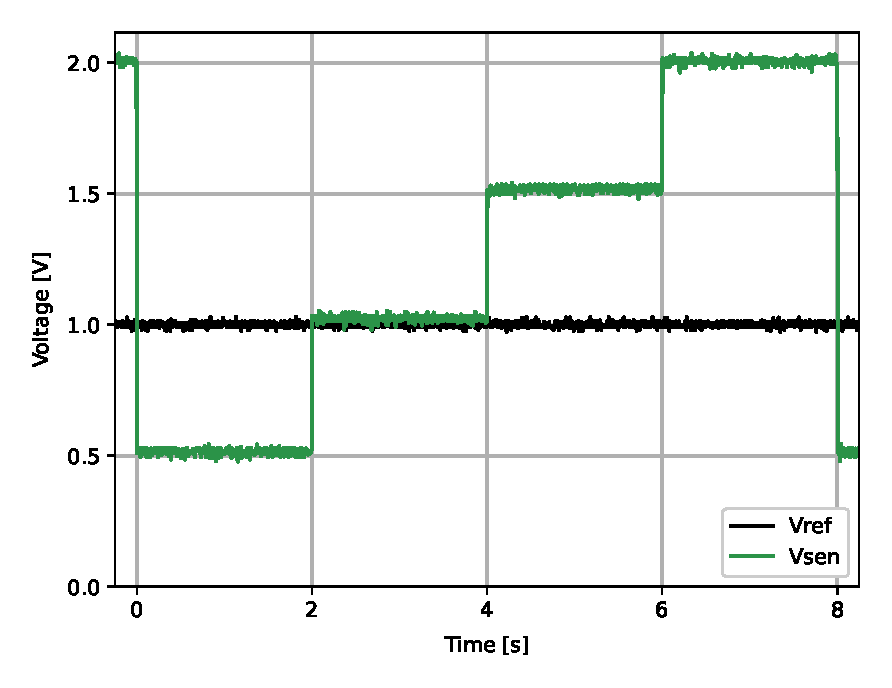
\includegraphics[width=.5\textwidth]{images/chapter_4/sensor_addressing/sensormux_ex.eps}
%    \caption{Sensor addressing functional test.}
%    \label{figure:sensormux-ex}
%\end{figure}

\begin{figure}[!ht]
    \centering
    \begin{minipage}{0.45\textwidth}
        \centering
        \includegraphics[clip, trim={0.1cm 6cm 22.9cm 5.7cm}, width=.65\textwidth]{images/front_pcb.pdf}
        \caption{3D view of the sensor addressing circuit in the PCB.}
        \label{figure:sensormux-pcb}
    \end{minipage}\hfill
    \begin{minipage}{0.45\textwidth}
        \centering
        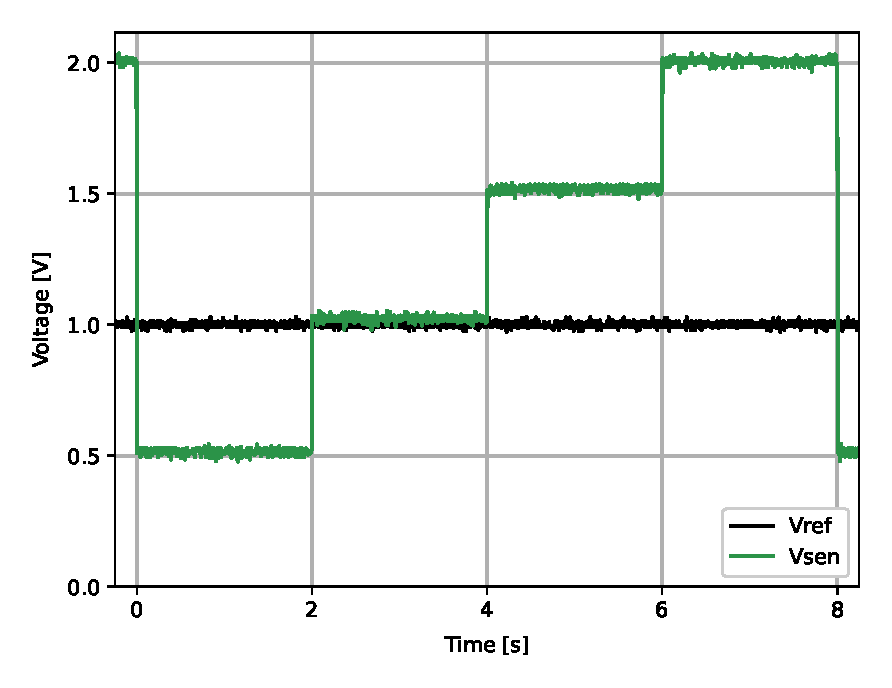
\includegraphics[width=\textwidth]{images/chapter_4/sensor_addressing/sensormux_ex.eps}
        \caption{Sensor addressing functional test.}
        \label{figure:sensormux-ex}
    \end{minipage}
\end{figure}

The use of multiplexers at the input stage offers opportunities for further exploration, whereby only one amplification scheme is required for multiple sensors. In this scenario, the input signals are multiplexed, reducing the overall size of the \ac{PCB} as a single amplification circuit suffices. However, incorporating input multiplexing introduces an additional layer of complexity, as the gains, settling times, and cut-off frequencies need to be adjusted accordingly. The $\mathrm{ADG1609}$ multiplexer used in this project has a settling frequency of $\mathrm{12.5~MHz}$, enabling the multiplexing of sensors at this frequency. Consequently, the \ac{HPF} at the inputs of the differential amplifier needs to be removed to accommodate the settling time of the signal. While this feature could have potential advantages in specific applications, it is not practical in the current context due to the influence of nominal resistance mismatch on the \ac{DC} component of the signal. The removal of the \ac{HPF} means that the \ac{DC} component, which is significantly higher than the \ac{AC} component, is not eliminated. As a result, there is a risk of saturation due to the amplified \ac{DC} component exceeding the amplifier's capabilities.

Figure \ref{figure:sensormux-pcb} illustrates the routing of the sensor addressing module. While only the traces on the top layer are visible, it should be noted that this module extensively utilizes all 4 layers for signal routing due to the significant number of different signals involved. The spacing between the headers has been carefully calculated to accommodate the attachment of the \ac{PCB} with the sensor chip to those headers.

% ----------------------------------------------------------------------------- Serial to Parallel Converter
\mytitle{Serial to Parallel Converter}

\noindent
In this work, multiplexers play a crucial role in addressing multiple sensors by enabling the selection of one input from multiple options and routing it to the desired output. However, during the development of this project, the availability of different multiplexing \ac{IC}s was significantly limited due to a semiconductor shortage. As a result, the project had to utilize the $\mathrm{ADG1609}$ multiplexer \ac{IC}.

The $\mathrm{ADG1609}$ device employs parallel communication, which means that data is transmitted simultaneously on multiple lines or bits. Consequently, the communication within the addressing module occurs through bits. To access a specific sensor, the multiplexers in the module receive binary signals as selection inputs. These signals determine which sensor is being accessed by setting the appropriate combination of bits.

Parallel communication through bits provides an advantage in terms of speed. However, it also introduces certain considerations regarding the number of inputs required to control each multiplexer. In the case of the chosen multiplexer \ac{IC}, the $\mathrm{ADG1609}$, it can only choose between 4 inputs. This means that to control each multiplexer, two control bits are needed in addition to the enable bit of the \ac{IC}. Considering that the addressing module comprises six multiplexers, with one dedicated to each channel, it results in a total of 18 inputs required to address and control all the sensors. This count includes the control bits and the enable bit for each multiplexer. However, it is worth mentioning that the enable bit may not be considered when counting the necessary inputs because the $\mathrm{ADG1609}$ \ac{IC} does not retain the configuration when enable is off. Thus, in practical terms, the addressing system would require a minimum of 12 inputs (6 multiplexers x 2 control bits), excluding the enable bit, to effectively control the multiplexers and access the desired sensor data.

Considering the specific requirements of your application, where high communication speeds in the selection of sensors are not crucial, it is feasible to optimize the addressing module by reducing the number of inputs. The reference voltage tuning module communicates using \ac{SPI}. By integrating the addressing module and the reference voltage tuning module, only one communication protocol needs to be programmed in the system software to control both modules. This simplifies the overall system architecture and eases the control process. The following solution uses shift registers to translate the \ac{SPI} information into parallel format.

\begin{figure}[!ht]
    \centering
    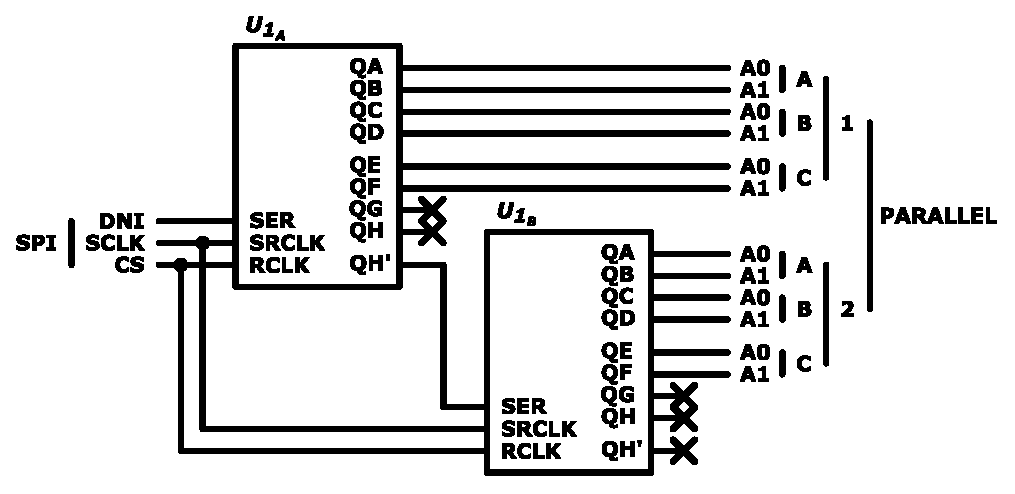
\includegraphics[width=.75\textwidth]{images/chapter_4/sensor_addressing/s2p.eps}
    \caption{Serial to parallel circuit (for more details refer to Appendix \ref{appendix:a}).}
    \label{figure:s2p}
\end{figure}

The circuit depicted in Figure \ref{figure:s2p} demonstrates the implementation of the serial to parallel module, which serves the purpose of converting the serial communication protocol, specifically \ac{SPI}, into a parallel format suitable for controlling the multiplexers. One of the advantages of this conversion is that it reduces the number of inputs required to control the multiplexers. In the \ac{SPI} format, only 3 inputs are needed to control the multiplexers, as these inputs are converted into 12 outputs, meeting the requirements of the 6 multiplexers. To achieve this conversion, the circuit utilizes shift registers. The shift registers effectively store and shift the incoming serial data bits ($SER$), allowing for the generation of parallel output signals ($Q_{A...H}$) that correspond to the desired sensor selections. The shift register clock ($SRCLK$) and the storage register clock ($RCLK$) are two essential signals in the operation of the circuit. The $SRCLK$ signal is responsible for controlling the shifting of data between the flip-flops within the \ac{IC}. When the $SRCLK$ signal transitions from one state to another, it triggers the sequential movement of data from one flip-flop to the next, effectively shifting the data along the shift register. On the other hand, the $RCLK$ signal is used to control the storage of the data present in each flip-flop into the output of the \ac{IC}. When the $RCLK$ signal changes state, it causes the outputs of the flip-flops to be latched into the storage register. The choice of the specific \ac{IC} used in the circuit design was not critical, and the widely popular $\mathrm{74HC595}$ shift register \ac{IC} was selected for the task. However, since the $\mathrm{74HC595}$ \ac{IC} only has 8 output pins available, it was necessary to utilize two of these \ac{IC}s to meet the requirements of the parallel communication. To address this limitation, the $\mathrm{74HC595}$ \ac{IC} incorporates a dedicated output pin ($Q_{H'}$) that is directly connected to the last flip-flop output within the shift register chain. This pin allows for cascading multiple devices together, expanding the available output capacity. In this configuration, the $Q_{H'}$ of the first \ac{IC} should be connected to the $SER$ pin of the second \ac{IC}. The previous explanation can be summarized in Figure \ref{figure:shiftregister}, which depicts the block diagram of the level shifters.

%\begin{figure}[!ht]
%    \centering
%    \includegraphics[clip, trim={0.1cm 15cm 23cm 1.8cm}, width=.5\textwidth]{images/front_pcb.pdf}
%    \caption{3D view of the serial to parallel circuit in the PCB.}
%    \label{figure:s2p-pcb}
%\end{figure}

\begin{figure}[!ht]
    \centering
    \begin{minipage}{0.475\textwidth}
        \centering
        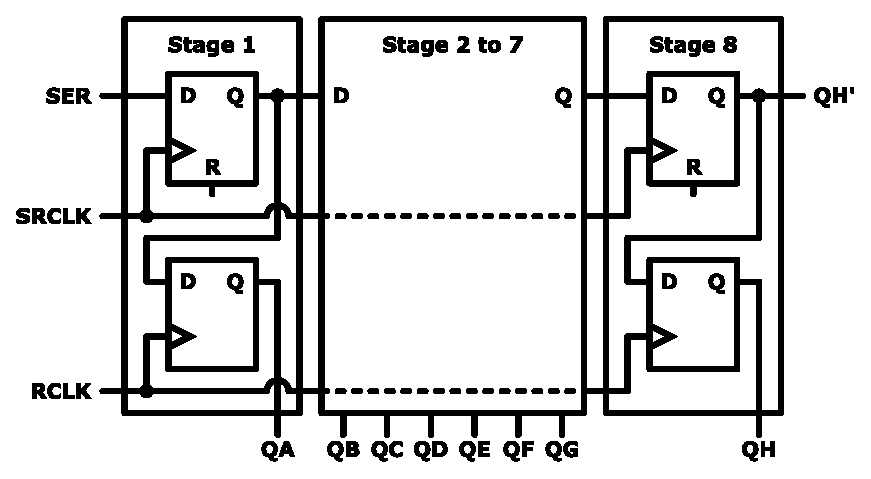
\includegraphics[width=\textwidth]{images/chapter_4/sensor_addressing/shiftregister.eps}
        \caption{Shift register functional block diagram.}
        \label{figure:shiftregister}
    \end{minipage}\hfill
    \begin{minipage}{0.475\textwidth}
        \centering
        \includegraphics[clip, trim={0.1cm 15cm 23cm 1.8cm}, width=.85\textwidth]    {images/front_pcb.pdf}
        \caption{3D view of the serial to parallel circuit in the PCB.}
        \label{figure:s2p-pcb}
    \end{minipage}
\end{figure}

Figure \ref{figure:s2p-pcb} presents the \ac{3D} representation of the serial to parallel circuit module. This module is positioned near the sensor addressing circuit, as its sole purpose is to convert serial communication into parallel form, enabling the functionality of the sensor multiplexer. In future versions of the cytometer platform, if the semiconductor shortage subsides and a wider range of multiplexer \ac{IC}s becomes available, it is recommended to use new multiplexers that can be controlled via \ac{SPI} and meet the specified requirements. In such cases, this module would become obsolete and should be removed to reduce board size. For consistency, this module is also shielded in line with other modules.
% ----------------------------------------------------------------------------- Serial to Parallel Converter
% ############################################################################# Sensor Addressing

% ############################################################################# Communication Translator
\section{Communication Translator}
\label{chapter:fe-comms}

The board designed in this work has been carefully equipped with multiple inputs and outputs to facilitate the seamless operation of the cytometer platform. Recognizing the importance of compatibility with various controlling or data acquisition systems that may interface with the \ac{PCB}, a circuit utilizing level shifters has been implemented. This design consideration ensures that the board can be effortlessly integrated into any system that requires control or data exchange. While this project specifically caters to a known system, it is worth noting that the level shifter circuit is not restricted solely to the DE-10 Standard \ac{FPGA} used as a real-time \ac{DSP} device. Its versatility allows for easy interfacing with other devices, as demonstrated by numerous tests conducted using an Analog Discovery or an Arduino. Therefore, regardless of the specific system or platform, the level shifter circuit can be readily employed to establish effective communication between components operating at different voltage levels, ensuring smooth and reliable functionality.

Level shifters, also known as voltage level translators, play a crucial role in providing signal separation between the device, specifically the \ac{FPGA} used in this work (DE-10 Standard), and the cytometer platform. The FPGA operates at a voltage level of $\mathrm{3.3~V}$, while the platform requires signals at either $\mathrm{5~V}$ or $\mathrm{2.5~V}$. In Figure \ref{figure:level-shifters}, the level shifter circuit is visually depicted as an integral part of the system. The figure provides a comprehensive overview of all the signals involved in transmitting or gathering information from the \ac{PCB}. Additionally, it illustrates the corresponding \ac{GPIO} pins that each signal represents for the DE-10 \ac{FPGA}. This graphical representation serves as a reference for understanding the signal flow and the role played by the level shifter circuit in maintaining signal integrity and compatibility between the \ac{FPGA} and the cytometer platform.

\begin{figure}[!ht]
    \centering
    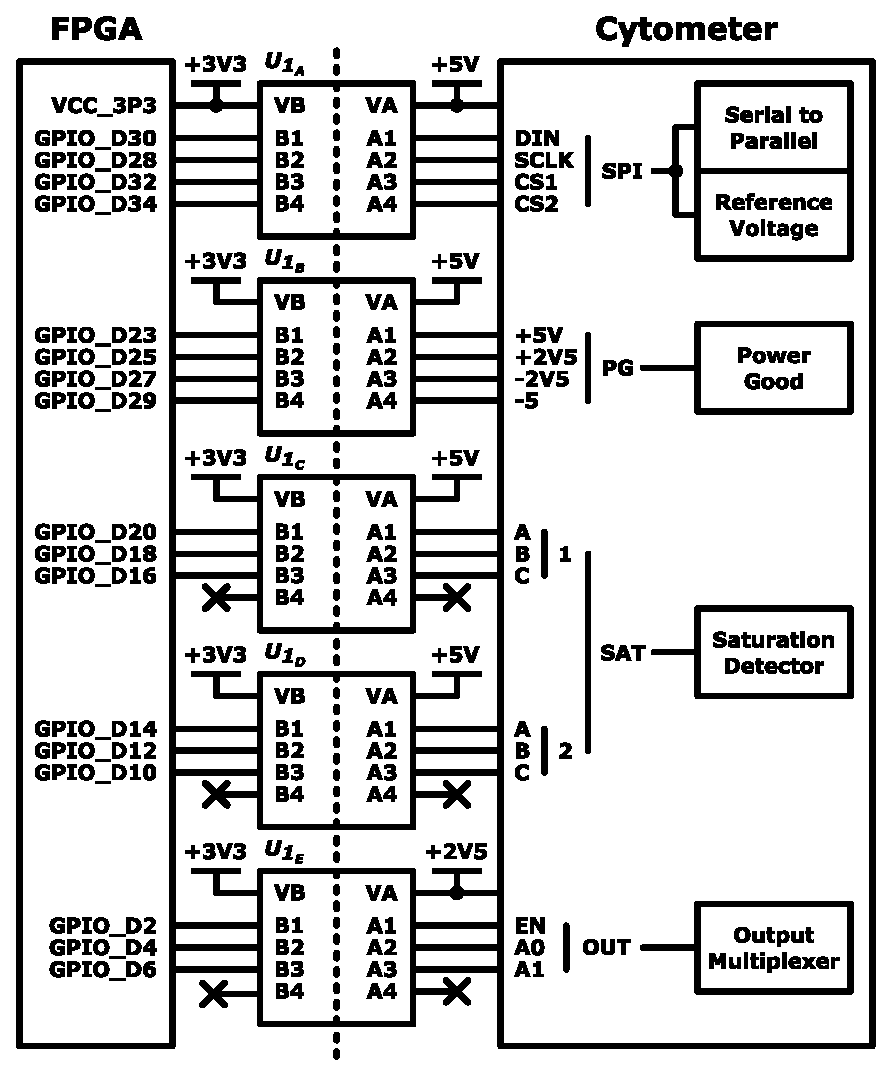
\includegraphics[width=.65\textwidth]{images/chapter_4/communications/comms.eps}
    \caption{Level shifters circuit (for more details refer to Appendix \ref{appendix:a}).}
    \label{figure:level-shifters}
\end{figure}

Figure \ref{figure:level-shifters} illustrates all the signals present on the \ac{PCB}. It is important to note that the voltage on side B of the level shifters is supplied by the interfaced device. In the depicted case, the $\mathrm{3.3~V}$ voltage is provided by the \ac{FPGA}, while the other voltages are supplied by the cytometer. The \ac{SPI} communication protocol will be utilized by two circuit blocks: the serial-to-parallel block and the reference voltage block. Each block operates with a distinct chip-select signal ($CS1$ and $CS2$). The serial-to-parallel block is responsible for converting the serial protocol into a set of bits that can be understood by the multiplexers in the sensor addressing circuit. Although the power good block has not been introduced yet, its purpose is to assess whether the supply rails have sufficient voltage to ensure the proper functioning of all the \ac{IC}s dependent on those rails. The \ac{FPGA} can utilize this information to verify if the cytometer is ready to receive instructions. The saturation detector block is designed to provide valuable information for the real-time \ac{DSP}. It allows the identification of a saturated signal during the amplification scheme, ensuring that such samples are not considered in subsequent processing steps. In the upcoming section, the output multiplexer module, which requires parallel communication to alternate between the channels' outputs, will be explained in detail.

\begin{figure}[!ht]
    \centering
    \includegraphics[clip, trim={23.2cm 7.1cm 0.6cm 7cm}, width=.5\textwidth]{images/front_pcb.pdf}
    \caption{3D view of the level shifter circuit in the PCB.}
    \label{figure:level-shifters-pcb}
\end{figure}

Figure \ref{figure:level-shifters-pcb} showcases the level shifter circuit integrated into the platform. This circuit comprises 5 level shifts housed within a larger \ac{RFI} shield, ensuring effective isolation from other modules. Although the \ac{PCB} does have a specific signal for all the 40 pins in the header, it is designed to be compatible with the DE-10 Standard \ac{GPIO} header. This compatibility simplifies the process of connecting the cytometer platform to the digital interface, eliminating the need for individual signal wiring.
% ############################################################################# Communication Translator

% ############################################################################# Output Multiplexing
\section{Output Multiplexing}
\label{chapter:fe-mux}

As mentioned earlier, the cytometer platform system was designed to ensure compatibility with a specific \ac{FPGA}, the DE-10 Standard \ac{FPGA}. However, the \ac{FPGA} itself lacks \ac{ADC}s necessary for signal acquisition. To address this limitation, a dedicated daughter board called the THDB-ADA was bought to provide a \ac{DSP} solution for the DE-series \ac{FPGA}s. This external module is also referred to as the "A/D and D/A Development Kit". The THDB-ADA card comes in two versions: one utilizing \ac{HSMC}, and the other utilizing \ac{GPIO}. Since the \ac{GPIO} header is already in use for information exchange between the platform and the \ac{FPGA}, the THDB-ADA card with the \ac{HSMC} connection was chosen. It's worth noting that both versions of the card are similar in functionality; their main difference lies in the type of connection header used. Although the kit includes both \ac{ADC}s and \ac{DAC}s, only the \ac{ADC}s are relevant for the specific application at hand. The purpose of the \ac{ADC}s is to capture the output signal generated by the analog channels, which will then undergo real-time \ac{DSP}. However, it should be noted that the card has a significant limitation in terms of the number of available \ac{ADC}s. While there are 6 different analog channels, the THDB-ADA itself only features 2 \ac{ADC}s. To address this challenge, a dedicated circuit was developed to multiplex the 6 channels into 2 outputs, effectively mitigating the issue.

Since the THDB-ADA card is equipped with 2 \ac{ADC}s and there are 2 primary channels, the most straightforward approach is to employ 1 multiplexer for each channel. These multiplexers will alternate between the outputs of 3 sub-channels that collectively encompass the main channel. The kit utilizes the $\mathrm{AD9248}$ \ac{ADC}s, known for their sampling rate of $\mathrm{65~MSPS}$ and a $\mathrm{2~V}$ peak-to-peak range. To ensure that the sampling rate limitation is imposed by the \ac{FPGA} and not the cytometer platform, it is necessary to employ multiplexers with a switching time faster than the sampling period of the \ac{ADC}s. Considering that these \ac{ADC}s will be shared among three sub-channels, the maximum achievable sampling rate per channel in this configuration is $\left(\nicefrac{65}{3}\right)\approx\mathrm{21~MSPS}$. However, it's important to note that there may also be scenarios where only one sub-channel is being acquired. In such cases, the sampling period is as low as $\mathrm{15~ns}$. When selecting the \ac{IC}, it is crucial to prioritize the scenario where only one sub-channel is being acquired to fully leverage the capabilities and benefits offered by the \ac{ADC}.

\begin{table}[ht]
    \centering
    \caption{Multiplexer ICs for the output multiplexing circuit.}
    \begin{small}
    \begin{tabular}{cccc}
\toprule
            & \begin{tabular}[c]{@{}c@{}}Switching Time \\ $t_{on}$ {[}ns{]}\end{tabular} & \begin{tabular}[c]{@{}c@{}}On Resistance\\ $R_{on}$ {[}$\Omega${]}\end{tabular} & Dual Supply {[}V{]} \\
\midrule
ADG409      & 85                                                                          & 40                                                                                           & $\pm 15$            \\
MC74HC4052A & 59                                                                          & 100                                                                                          & $\pm 6$             \\
ADG709      & 14                                                                          & 3                                                                                            & $\pm 2.5$           \\
ADG759      & 14                                                                          & 3                                                                                            & $\pm 2.5$           \\
\bottomrule
\end{tabular}
    \end{small}
    \label{tab:outmux-ic}
\end{table}

Table \ref{tab:outmux-ic} illustrates the available multiplexers at the time of selection, taking into account the semiconductor shortage previously mentioned in the sensor addressing module. The presented multiplexers in the table are chosen for their minimal switching time. Since speed is a critical factor for this circuit, the communication protocol used to control the multiplexers is not relevant. Therefore, all of the multiplexers are controlled using parallel communication. Additionally, the supply voltage needs to be considered since the signal is no longer referenced to the ground due to the removal of the \ac{DC} component in the sensor response signal. Among the options, the $\mathrm{ADG409}$ and $\mathrm{MC74HC4052A}$ appeared promising as their supply voltage matched the power lines required for each \ac{IC} on the board. However, their switching times were not fast enough, and not even the scenario where all 3 sub-channels are acquired simultaneously, sampling period of $\mathrm{46~ns}$, would fully benefit from the \ac{ADC}s' potential. As a result, the choice was narrowed down to the $\mathrm{ADG709}$ and $\mathrm{ADC759}$, both offering identical performance. The selection was primarily based on the footprint, and the $\mathrm{ADG709}$ had the most commonly used footprint, making it easier to replace with another \ac{IC} if needed. One drawback of using this multiplexer is that the power circuit needs to be designed to accommodate additional supply rails to power this \ac{IC}. The output multiplexing circuit, employing these multiplexers, is depicted as follows:

\begin{figure}[!ht]
    \centering
    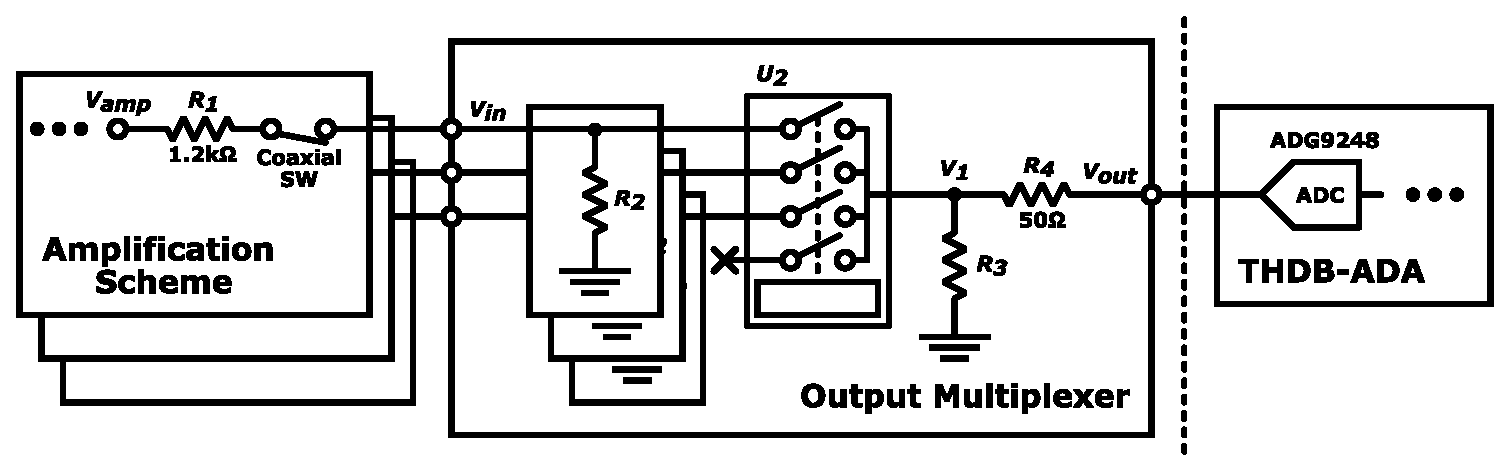
\includegraphics[width=.9\textwidth]{images/chapter_4/communications/outmux.eps}
    \caption{Output multiplexer circuit (for more details refer to Appendix \ref{appendix:a}).}
    \label{figure:outmux}
\end{figure}

The circuit depicted in Figure \ref{figure:outmux} showcases the implementation of output multiplexing in the developed cytometer platform. It is worth noting that the picture only represents a single channel, but it should be understood that this circuit is replicated twice to cater to the presence of two channels in total. Moreover, the $\mathrm{ADG709}$ features an input voltage protection mechanism. If any of the inputs surpasses the maximum or minimum supply voltage, the \ac{IC} will activate clamping, effectively shutting down. In such a scenario, crosstalk may occur between the selected channel and the input signal that exceeded the supply voltage due to clamping. Hence, it is essential for the circuit to ensure that the input signals do not exceed the range of  $\mathrm{\pm~2.5~V}$, and the output should not exceed $\mathrm{\pm~1~V}$ range. This output limitation is necessary because the \ac{FPGA} \ac{ADC} is not capable of handling higher voltages, as specified before. The voltage reduction is achieved within this module, and not considered in the amplification scheme gain. This design approach allows for compatibility with the previous version of the cytometer, utilizing the same \ac{ADC} and ensuring broader compatibility beyond just \ac{FPGA} usage. The voltage reduction is achieved through a two-step process using voltage dividers. Equations \ref{equation:outmux-vin} and \ref{equation:outmux-vout} represent the specific calculations for this reduction.
\begin{equation}
    v_{in} = \frac{R_{2}}{R_{1}+R_{2}} \cdot v_{amp}\; \left(< \pm~2.5~\mathrm{V}\right) \quad [\mathrm{V}]
    \label{equation:outmux-vin}
\end{equation}
\begin{equation}
    v_{out} = \frac{R_{2}//R_{3}}{R_{1}+R_{2}//R_{3}} \cdot v_{amp}\; \left(< \pm~ 1~\mathrm{V}\right) \quad [\mathrm{V}]
    \label{equation:outmux-vout}
\end{equation}

\noindent
Both Equations \ref{equation:outmux-vin} and \ref{equation:outmux-vout} are referenced to $v_{amp}$, which represents the signal obtained from the amplification scheme immediately after the filter stage. As previously mentioned, the filter can't drive a signal higher than $\mathrm{\pm 4.5~V}$. The voltage divider takes into account the minimum load resistance ($R_1$) required by the \ac{LPF}. In Equation \ref{equation:outmux-vout}, the calculation despises the impact of the $R_{on}$ of the multiplexer and the impedance matching resistor ($R_4$). These resistances are relatively low, and their effect on the result is negligible. The voltage divider to address the specified limitations, employees resistors $R_2$ and $R_3$, both with a value of $\mathrm{680~\Omega}$. The functionality of these resistors and the role of the multiplexing circuit can be illustrated in Figure \ref{figure:outmux-func}.

%\begin{figure}[!ht]
%    \centering
%    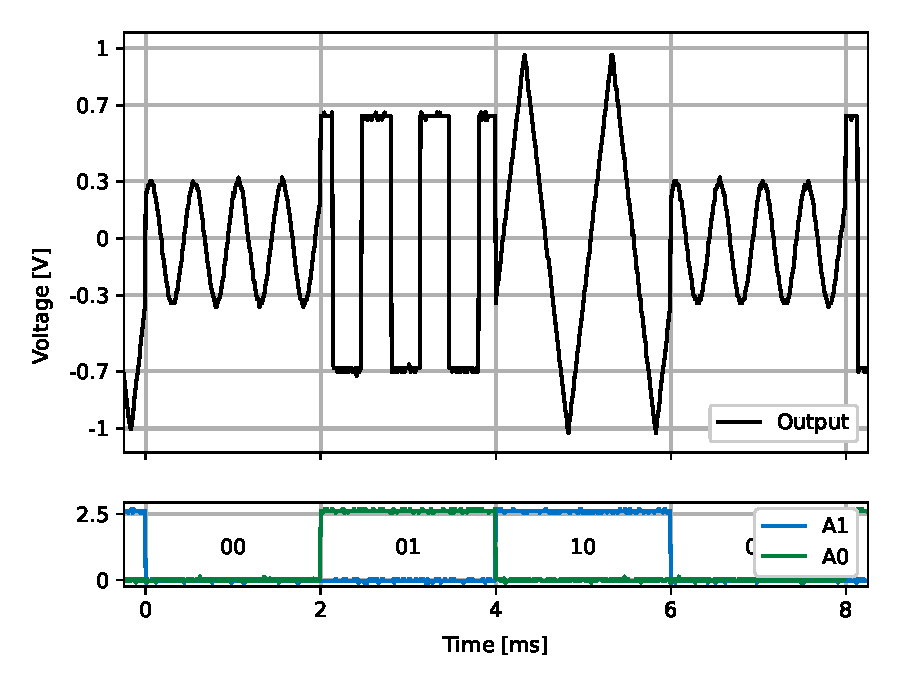
\includegraphics[width=.5\textwidth]{images/chapter_4/communications/outmux_ex.eps}
%    \caption{Output multiplexer functional test.}
%    \label{figure:outmux-func}
%\end{figure}

\begin{figure}[!ht]
    \centering
    \begin{minipage}{0.45\textwidth}
        \centering
        \includegraphics[clip, trim={18.8cm 13.3cm 0.2cm 1.8cm}, width=.99\textwidth]{images/front_pcb.pdf}
        \caption{3D view of the output multiplexer circuit in the PCB.}
        \label{figure:outmux-pcb}
    \end{minipage}\hfill
    \begin{minipage}{0.45\textwidth}
        \centering
        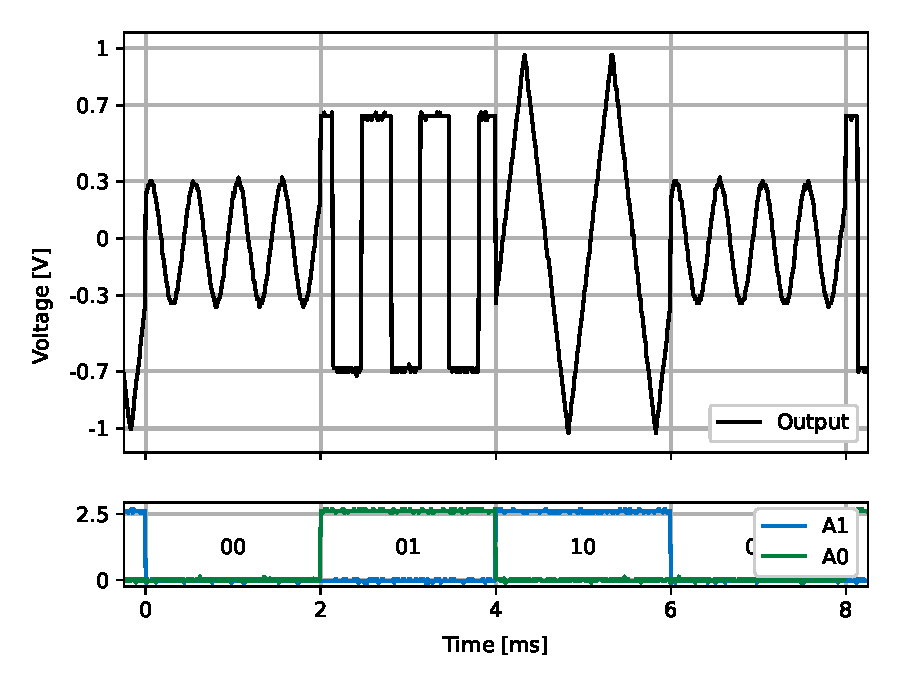
\includegraphics[width=\textwidth]{images/chapter_4/communications/outmux_ex.eps}
        \caption{Output multiplexer functional test.}
        \label{figure:outmux-func}
    \end{minipage}
\end{figure}

Figure \ref{figure:outmux-func} illustrates a test conducted to evaluate the performance of the circuit in multiplexing three known signals, simulating the behavior of the sensors. This test was performed using an Analog Discovery device and an oscilloscope. During the test, a sine wave with a frequency of $\mathrm{2~kHz}$ and amplitude of $\mathrm{\pm 1.5~V}$ was generated by the oscilloscope and connected to the first input of the circuit, represented by the word "00". Additionally, a square signal with a frequency of $\mathrm{1.5~kHz}$ and amplitude of $\mathrm{\pm 3~V}$, was applied to the second input, represented by the word "01". Furthermore, a triangular signal with a frequency of $\mathrm{1~kHz}$ and amplitude of $\mathrm{\pm 4.5~V}$ was fed into the third input, represented by the word "10". A resistor with $\mathrm{1.2~k\Omega}$ value, was also added in series to the input signals to mimic ($R_1$). The control sequence was generated using Analog Discovery. The circuit is confirmed to be functional as the signals applied at the input are observed at the output, with the expected reduction in amplitude. The amplitude reduction can be calculated using Equation \ref{equation:outmux-vout}.
\begin{equation}
    \nonumber v_{out1_{max}} = \frac{680//680}{1.2k+680//680} \cdot 1.5 \approx 0.33~\mathrm{V}\;;\quad v_{out2_{max}} \approx 0.66~\mathrm{V}\;;\quad v_{out3_{max}} \approx 0.99~\mathrm{V}
\end{equation}

Figure \ref{figure:outmux-pcb} showcases the output multiplexer circuit as a module that has been integrated into the cytometer \ac{PCB}. This module is designed to function independently, with inputs being connected through SMA connectors. The amplification scheme can be detached from this circuit using the coaxial switches mentioned in the relevant section. This unique feature allows this module to be utilized as a mini-board for other applications or even with the previous cytometer platform, which can be cascaded for redundant measurements. In such a scenario, the \ac{FPGA} or other \ac{DSP} interfaces can be employed for data processing.
% ############################################################################# Output Multiplexing

% ############################################################################# Power
\section{Power Supply}
\label{chapter:fe-power}

In the realm of electronic circuits, all the circuitry explained in this chapter relies on a reliable and adequate power supply to ensure proper functioning. Power is of utmost importance in electronic circuits as it provides the necessary energy for the correct operation of circuit components, enabling the generation and propagation of desired electrical signals and functionalities. This section focuses on the critical aspect of power in electronic circuits. In the upcoming sections, a detailed exploration of power circuits will be undertaken. A comprehensive understanding of power circuits is vital for achieving optimal performance, reliability, and longevity of the electronic system.

To ensure the proper functioning of the cytometer platform, four supply rails are required. The board must be capable of providing the following voltages: $\mathrm{+5~V}$, $\mathrm{+2.5~V}$, $\mathrm{-2.5~V}$, and $\mathrm{-5~V}$. In order to enhance flexibility, the circuit was designed to accommodate multiple power sources. The first power source utilized is batteries, which were also employed in the previous platform. Battery power offers reliability, minimal noise introduction, and portability, making it an ideal choice for experiments and field use. This enables the system to be self-contained and independent of external power sources. As an alternative to batteries, a laboratory \ac{DC} power supply can be used. However, it is important to note that this power supply may introduce higher levels of noise compared to batteries. Additionally, the portable aspect is compromised, as the system becomes reliant on a stationary power source. The third power source is the \ac{FPGA} itself. The cytometer platform is designed to be compatible with the DE-10 Standard \ac{FPGA}, simplifying the setup process and the required equipment. By utilizing the power supply provided by the \ac{FPGA}, the system benefits from a streamlined configuration and reduced complexity. Lastly, \ac{USB} power can also serve as a power source for the cytometer platform. This allows for the use of power banks or even direct connections to a computer running the cytometer software. \ac{USB} power is convenient as a computer is required to configure and control all necessary parameters prior to usage. By accommodating these three power sources, the cytometer platform offers flexibility and adaptability to different operating scenarios. Users can choose the most suitable power source based on their specific needs.

\begin{figure}[!ht]
    \centering
    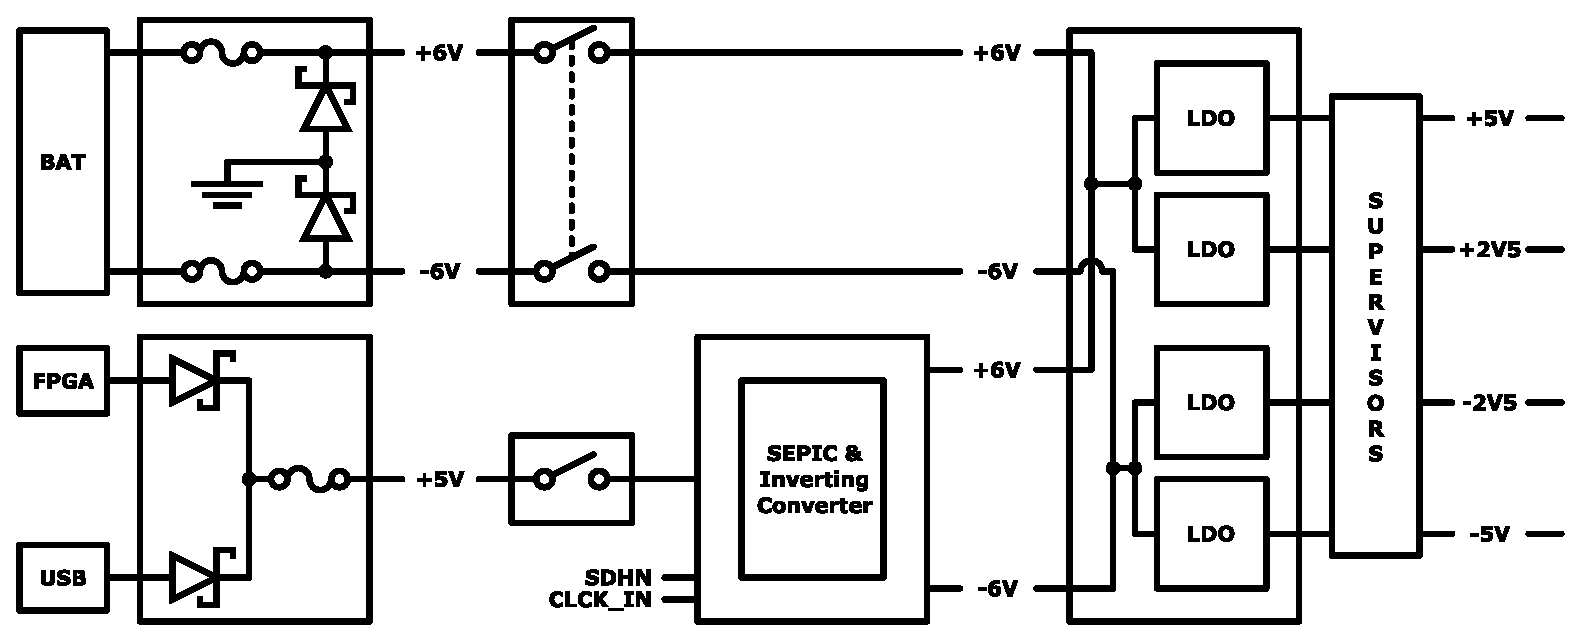
\includegraphics[width=.85\textwidth]{images/chapter_4/power/power.eps}
    \caption{Power circuit diagram (for more details refer to Appendix \ref{appendix:a}).}
    \label{figure:pwr-sources}
\end{figure}

Figure \ref{figure:pwr-sources} illustrates the block diagram showcasing the transformation of power sources into the necessary power rails for the \ac{PCB}. Several measures are implemented to ensure the safe and efficient utilization of these power sources. To protect against mistakes when connecting the battery, a power protection circuit is employed. This circuit safeguards the subsequent \ac{IC}s by preventing damage, and in case of any fault, only a fuse needs to be replaced. To prevent current flow between the \ac{FPGA} and \ac{USB} power supplies when both are connected, a Schottky diode is utilized. This diode ensures the isolation of the power sources, avoiding potential issues that may arise from simultaneous connection. Since the \ac{FPGA} and \ac{USB} power sources provide a fixed \ac{DC} voltage, a \ac{DC}/\ac{DC} is necessary. In this application, a \ac{SEPIC} and inverting circuit is used to boost the signal to ensure proper functionality of the following circuitry. Additionally, its inverting feature generates an inverted voltage, resulting in two power rails. The outputs of the \ac{SEPIC} and inverting converter circuit mimic the battery power supply, providing $\mathrm{\pm 6~V}$ rails. Lastly, an \ac{LDO} regulator circuit is employed to adjust the input voltage to meet the specific requirements of the \ac{PCB}. This ensures a stable and reliable power supply for the circuit components. By implementing these power conversion and protection mechanisms, the \ac{PCB} can efficiently utilize the available power sources and provide the necessarily regulated voltages for the proper functioning of the circuitry.

\begin{table}[ht]
    \centering
    \caption{Supply current requirements of the components in the cytometer platform.}
    \begin{small}
    \begin{tabular}{ccccc}
\toprule
\multirow{2}{*}{Module}               & \multirow{2}{*}{Component} & \multirow{2}{*}{Quantity} & \multicolumn{2}{c}{Supply Current {[}mA{]}} \\
\cmidrule(r){4-5}
                                      &                            &                           & Typical              & Maximum              \\
\midrule
\multirow{2}{*}{Bias Topology}        & LT1677                     & 6                         & 2.6                  & 3.4                  \\
                                      & Mirror Branch              & 12                        & 1                    & 5                    \\
\multirow{2}{*}{Reference Voltage}    & ADR444                     & 1                         & 3                    & 3.75                 \\
                                      & AD5676                     & 1                         & 1.1                  & 1.26                 \\
\multirow{3}{*}{Amplification Scheme} & AD8429                     & 6                         & 6.7                  & 7                    \\
                                      & LT1677                     & 6                         & 2.6                  & 3.4                  \\
                                      & LTC1563-2                  & 6                         & 15                   & 23                   \\
Saturation Detector                   & LM2901                     & 6                         & \num{2.5e-2}         & \num{2.5e-1}         \\
Sensor Addressing                     & ADG1609                    & 6                         & \num{1e-6}           & \num{1e-3}           \\
Serial to Parallel                    & 74HC595                    & 2                         & \num{1e-7}           & \num{1e-4}           \\
Communication                         & LSF0204-Q1                 & 5                         & \num{2.5e-3}         & \num{5e-3}           \\
Power Supervisors                     & TLV809                     & 4                         & \num{1.6e-2}         & \num{1.7e-2}         \\
\midrule
                                      &                            & Total:                    & 178                  & 288                  \\
\bottomrule
\end{tabular}
    \end{small}
    \label{tab:pwr-consumption}
\end{table}

Table \ref{tab:pwr-consumption} provides a rough overview of the power consumption for each individual \ac{IC} within the various modules of the platform. Upon observation, it can be noted that the new features have a relatively low impact on the supply current. However, the most significant factor contributing to the increased current demand is the expanded number of analog channels, which is three times greater than that of the previous platform. These values were obtained from the respective datasheets of each component. To ensure the proper functioning of the system, it is important to consider the worst-case scenario where all components are operating at their maximum power consumption. In order to meet the power demands of the system, the \ac{LDO} regulator circuit must be designed to provide the required supply current, in that scenario.

% ----------------------------------------------------------------------------- Low-Dropout Regulators
\mytitle{Low-Dropout Regulators}

\noindent
The \ac{LDO} regulators circuit was designed to ensure the stability of power rails throughout the platform's electronic circuits. The inclusion of \ac{LDO} regulators is essential for maintaining a consistent and precise output voltage, regardless of variations in the input voltage or changes in the load. Additionally, \ac{LDO} regulators, as the name implies, have a low dropout voltage. This characteristic denotes the minimum voltage difference between the input and output voltages at which the regulator can maintain proper regulation. The low dropout voltage enables \ac{LDO} regulators to operate efficiently even when the input voltage is close to the desired output voltage. As a result, power utilization is maximized, and the circuits can perform optimally. One of the key advantages of \ac{LDO} regulators is the built-in filtering and noise reduction mechanisms. These features effectively suppress high-frequency noise and ripple present in the input power source, ensuring a cleaner and more reliable output voltage for sensitive components. By mitigating noise interference, \ac{LDO} regulators contribute to improved performance and enhanced reliability of the circuits. Their design and integration into the circuitry are relatively simple, making them a practical choice for power rail stabilization.

Due to the limited availability of \ac{LDO} regulator \ac{IC}s, the selection process for the appropriate \ac{IC} was primarily based on the required supply current, which needed to exceed $\mathrm{288~mA}$ as indicated in Table \ref{tab:pwr-consumption}. Additionally, the chosen \ac{IC} had to be capable of providing the necessary voltages of $\mathrm{+5~V}$, $\mathrm{+2.5~V}$, $\mathrm{-2.5~V}$, and $\mathrm{-5~V}$. To streamline the design and enhance simplicity, an \ac{IC} with adjustable output voltage was preferred, allowing for the possibility of using the same \ac{IC} and circuit configuration to fulfill all the required voltage specifications. The \ac{LDO} regulators from Analog Devices, specifically the $\mathrm{LT3045\textnormal{-}1}$ \ac{IC} for $\mathrm{+5~V}$ and $\mathrm{+2.5~V}$ and the $\mathrm{LT3094}$ \ac{IC} for $\mathrm{-5~V}$ and $\mathrm{-2.5~V}$, were chosen for this purpose. These regulators not only fulfilled the voltage requirements but also featured ultra-low noise, a $\mathrm{500~mA}$ output current that could be limited, adjustable output voltages, and programmable power good functionality. Since the selected \ac{LDO} regulators provided significantly more current than required, the $\mathrm{5~V}$ rails were limited to $\mathrm{350~mA}$ and the $\mathrm{2.5~V}$ rails to $\mathrm{50~mA}$ to ensure efficient operation within the desired limits.

\begin{figure}[!ht]
    \centering
    \includegraphics[clip, trim={18.8cm 2cm 6.1cm 13.4cm}, width=.35\textwidth]{images/front_pcb.pdf}
    \caption{3D view of the LDO regulators circuit in the PCB.}
    \label{figure:ldo-pcb}
\end{figure}

Figure \ref{figure:ldo-pcb} depicts the routing of the \ac{LDO} regulators circuit, showcasing the separation of each power rail. The implementation of the power good feature can be observed, denoted by the centrally positioned \ac{LED}s. These \ac{LED}s serve to indicate when the voltage drops below predefined thresholds, such as $\mathrm{1.55~V}$ for the $\mathrm{2.5~V}$ rails and $\mathrm{4.05~V}$ for the $\mathrm{5~V}$ rail. Although this feature is redundant given the presence of a supervisor circuit, which will be discussed later in the document, it was incorporated within the design to utilize the available space within the \ac{RFI} shield. Furthermore, the circuit features potentiometers located on the sides, enabling precise adjustment of the output voltage.
% ----------------------------------------------------------------------------- Low-Dropout Regulators

% ----------------------------------------------------------------------------- SEPIC and Inverting Converter
\mytitle{SEPIC and Inverting Converter}

\noindent
The \ac{LDO}s are commonly used in situations where the voltage difference between the input and output is small. In these cases, the input voltage must be higher than the output voltage to ensure proper regulation. However, this requirement becomes a limitation when the power supplies are derived from the \ac{FPGA} or the \ac{USB}, which provide a fixed $\mathrm{+5~V}$ voltage. To overcome this limitation, a \ac{SEPIC} converter circuit is implemented. This particular type of \ac{DC}/\ac{DC} converter enables stepping up the input voltage obtained from these sources, addressing the issue effectively. In addition to the required voltage boost, the \ac{LDO}s circuit also relies on a negative voltage. Thus, besides the \ac{SEPIC} circuit, an inverting circuit is also required. These types of circuits, as the name implies, are able to generate a negative voltage from a positive input voltage. The purpose of this module is to combine both these \ac{DC}/\ac{DC} converters to mimic the batteries' power supply. 

To simplify the circuitry in this module, the $\mathrm{LT8582}$ \ac{DC}/\ac{DC} converter was chosen. This converter offers the desired functionalities, serving as a \ac{SEPIC} by generating an output voltage higher than the input while also providing the capability to invert the polarity of the input. As a result, it facilitates the provision of two boosted power rails with inverted polarity, thereby meeting the requirements of the system. The integration of this \ac{IC} significantly streamlined the overall design process. The output voltage of the $\mathrm{LT8582}$ converter is adjustable, relying on the nominal values of the components used. The equations necessary to achieve the desired output voltage can be found in the datasheet of the \ac{IC}, providing flexibility in configuring the output to meet specific requirements. In order for the $\mathrm{LT8582}$ to generate the desired output voltages, it requires a clock signal. The \ac{IC} offers the option to either generate an internal clock or utilize an external clock source. However, it's worth noting that using the internal clock may introduce additional noise to the output voltage. To mitigate this noise and ensure a cleaner power supply, it is recommended to utilize an external clock signal that should be synchronous or even shared with the \ac{ADC}s acquisition clock. This synchronization helps to minimize the impact of ripple noise on the system, leading to improved overall performance.

\begin{figure}[!ht]
    \centering
    \includegraphics[clip, trim={23.35cm 2.8cm 2.5cm 13.4cm}, width=.35\textwidth]{images/front_pcb.pdf}
    \caption{3D view of the SEPIC and inverting converter circuit in the PCB.}
    \label{figure:boost-pcb}
\end{figure}

Figure \ref{figure:boost-pcb} illustrates the \ac{3D} model of the implemented \ac{SEPIC} and inverting converter circuit. The routing of this module was executed with simplicity, following the guidelines provided in the \ac{IC} datasheet. The clear documentation and recommendations in the datasheet greatly facilitated the routing process, ensuring an efficient, reliable and compact layout inside the \ac{RFI} shield. In addition to the primary functionalities, the $\mathrm{LT8582}$ converter incorporates a shutdown pin. This pin offers the convenience of controlling the cytometer platform through software, eliminating the need for manual switch operation. By utilizing the shutdown pin, the system can be easily powered on or off as required, providing enhanced user control.

% ----------------------------------------------------------------------------- SEPIC and Inverting Converter
% ----------------------------------------------------------------------------- Power Supervisors
\mytitle{Power Supervisors}

\noindent
Given the vital role of power in any hardware equipment, it is essential to incorporate a circuit that constantly monitors the voltage levels of power supplies. This circuit serves to detect under-voltage and over-voltage conditions, enabling the user to ensure that the voltage remains within the specified range. Maintaining the voltage within the proper range is critical for the reliable operation of sensitive electronic components, preventing malfunctions or damage caused by insufficient or excessive voltage. To address this requirement, a power supervisor circuit was implemented in the cytometer platform \ac{PCB}. This circuit offers valuable features such as fault detection for over-current, short circuits, and thermal issues. By promptly identifying and addressing faults, the power supervisor circuit enhances the safety and integrity of the system. Additionally, it provides important feedback to users or system controllers, relaying vital information about power supply status and diagnostics. The power supervisor circuit in the cytometer platform \ac{PCB} adds an extra layer of protection and user awareness, ensuring that power supply conditions are monitored and potential issues are detected in a timely manner.

The circuit implemented in this work shares similarities with the previous design, as it utilizes the same family of supervisor \ac{IC}s for monitoring the power rails. However, there are notable differences in this iteration. Instead of using a supervisor \ac{IC} with an open-drain output, a push-pull output version is employed, eliminating the need for an additional pull-up resistor. Moreover, due to the increased number of power rails in the system, a greater quantity of supervisor \ac{IC}s is now required. The chosen supervisor \ac{IC}, the $\mathrm{TLV809}$, offers a wide range of threshold voltage options. However, it is important to note that the threshold voltage cannot be adjusted. Therefore, careful consideration is necessary to choose the appropriate \ac{IC} with the desired threshold voltage that aligns with the system requirements.

Although not deemed mandatory for the overall functionality of the cytometer, the power supervisor module still holds significance. While not extensively studied, the same \ac{IC}s were utilized in this module, as they effectively detect under-voltage conditions. In this particular case, threshold voltages of $\mathrm{4.55~V}$ and $\mathrm{2.25~V}$ were employed. However, for future iterations of the board, the circuitry in this module could be further improved to encompass the detection of both under-voltage and over-voltage scenarios. Nonetheless, given the multitude of new features implemented in this work's board, this particular feature was considered non-critical at this stage.

\begin{figure}[!ht]
    \centering
    \begin{minipage}{0.45\textwidth}
        \centering
        \includegraphics[clip, trim={18.2cm 11.9cm 7.3cm 7cm}, width=.99\textwidth]{images/back_pcb.pdf}
        \caption{3D view of the power supervisors circuit in the PCB.}
        \label{figure:supervisors-pcb}
    \end{minipage}\hfill
    \begin{minipage}{0.45\textwidth}
        \centering
        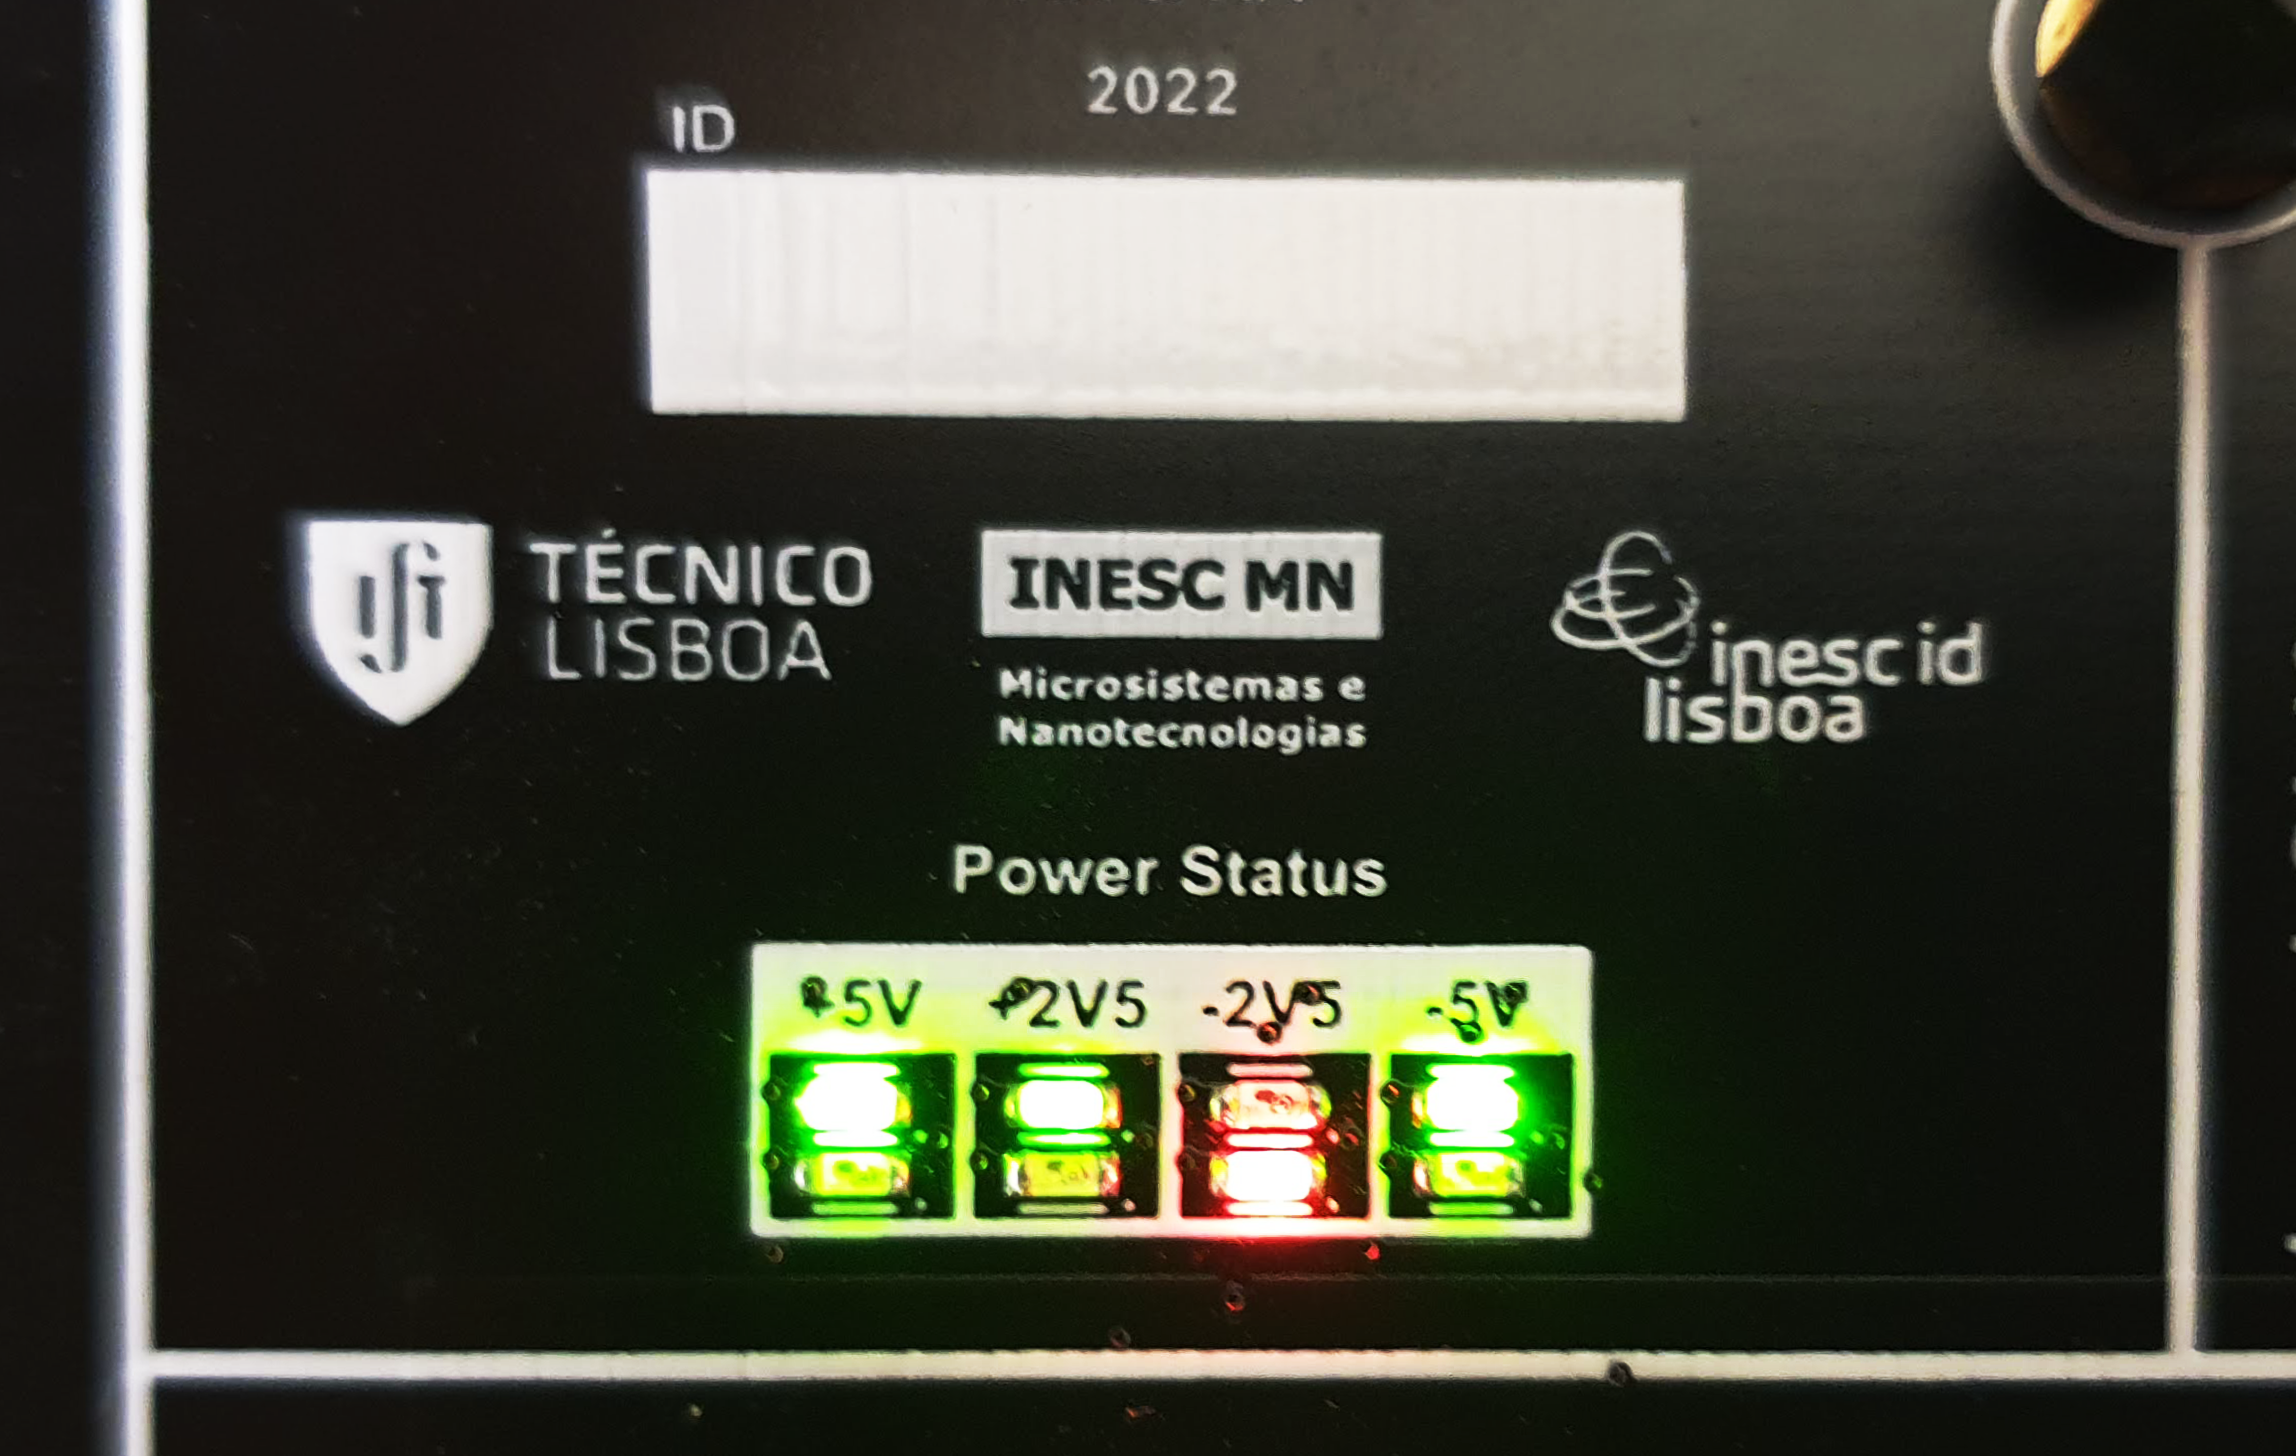
\includegraphics[width=\textwidth]{images/chapter_4/power/supervisors.png}
        \caption{Power supervisors LED display with $\mathrm{-2.5~V}$ rail under threshold voltage.}
        \label{figure:supervisors-func}
    \end{minipage}
\end{figure}

Figure \ref{figure:supervisors-func} showcases the functionality of the supervisor circuit by providing valuable feedback to users through the \ac{LED}s indicators. It is worth highlighting that the signals indicating which \ac{LED} (green or red) is illuminated are also accessible to the system operating the cytometer platform (e.g., \ac{FPGA}). This feature allows the cytometer software to wait for the \ac{IC}s to receive sufficient supply voltage before sending instructions, ensuring optimal performance. A notable observation from the figure is that the $\mathrm{-2.5~V}$ power rail is experiencing an issue. By deliberately adjusting the output voltage of this \ac{LDO} rail to a value above $\mathrm{-2.25~V}$, the supervisor \ac{IC} is triggered. This configuration demonstrates the circuit's functionality in detecting and indicating deviations from the desired voltage range.

The \ac{3D} routing and placement of the components in this module can be observed in Figure \ref{figure:supervisors-pcb}. The module was positioned on the bottom layer of the \ac{PCB}, directly underneath the \ac{LED} display depicted in Figure \ref{figure:supervisors-func}.
% ----------------------------------------------------------------------------- Power Supervisors
% ############################################################################# Power

% ############################################################################# Discussion and Results

\section{Discussion and Results}
\label{chapter:fe-results}

This chapter offers a comprehensive exploration and analysis of the circuitry employed in the cytometer platform. The current study incorporates a range of novel features designed to overcome limitations identified in the previous platform. By conducting rigorous testing and evaluation, the results obtained provide valuable insights into the enhanced performance and effectiveness of the cytometer platform. This section delves into a detailed discussion, highlighting the achieved accomplishments, while also presenting overall results related to system performance in terms of noise and magnetic field detection.

The analog path in the current platform follows a similar design to the previous iteration. In order to induce changes in resistance when exposed to a magnetic field, the passive sensors require a biasing current. This current is generated by the biasing architecture, which incorporates two distinct topologies within the same module. The first topology involves placing the sensors outside the feedback loop (open-loop), a configuration commonly employed in various other platforms. The second topology entails placing the sensors inside the feedback loop (closed-loop), enabling the op-amp to eliminate noise introduced by the components. It is worth noting that while the implementation of the closed-loop topology falls outside the scope of this thesis, it presents an avenue for future studies. Each of these topologies possesses its own characteristics. The open-loop topology offers a current independent of the sensor's resistance, making it easier to stabilize and allowing for the branching of current into multiple sensors. On the other hand, the closed-loop topology exhibits a current dependent on the sensor's load resistance, making stabilization more challenging. However, it offers a significant advantage in effectively canceling out noise from various sources, except for the reference voltage and the op-amp. The biasing architecture in both topologies relies on a reference voltage that determines the current supplied to the sensors. In this version, a \ac{DAC} is implemented to provide the reference voltage, allowing for software control instead of manual adjustment using a potentiometer. In addition to the biasing architecture, the analog path includes an amplification scheme that plays a crucial role in reducing quantization noise associated with digital conversion. This module amplifies the signal from the hundreds of $\mathrm{\mu V}$ to the units of $\mathrm{V}$ range, thereby maximizing the dynamic range of the \ac{ADC}s. Furthermore, this module incorporates a filter to prevent aliasing in the digital signal. The filter's primary purpose is to eliminate undesired frequency components that could distort or corrupt the signal during the analog-to-digital conversion process.

The \ac{MR} sensors utilized in this study were fabricated at \ac{INESC-MN}, resulting in a chip containing 28 different \ac{MR} sensors. To effectively utilize the capabilities of these sensors, a sensor addressing circuit was developed. The purpose of this module is to enable each of the six analog channels to select from a pool of four sensors available on the chip. This provides various opportunities for experimentation and analysis. For example, consider a scenario where two sensors within the same microfluidic channel are utilized for redundant measurements. If a magnetic particle induces a resistance change in both sensors simultaneously, it can be inferred that a particle has indeed passed through the channel, as opposed to being an external interference. Furthermore, envision a situation where three sensors are employed, with one placed in a microfluidic channel that does not have any sample flowing through it, serving as a reference channel. By utilizing the common noise present in all three sensors, optimal particle detection can be achieved by effectively removing the noise component. One limitation of this module relates to the communication requirements for controlling the multiplexers responsible for sensor selection through software. Due to the constraints imposed by the semiconductor shortage during the time of this work, the parallel control of the multiplexers requires an excessive number of inputs. However, to address this issue, a communication translator to \ac{SPI} was employed. This translator effectively reduced the number of inputs required while ensuring compatibility with the communication protocol used by the reference voltage module. 

In addition to the analog path, the design of the frontend interface also considered the digital path. Even though, the digital aspect falls beyond the scope of this thesis and is addressed in another thesis that utilizes a THDB-ADA card for signal acquisition and a DE-10 Standard \ac{FPGA} for real-time signal processing. To overcome the limitations of the \ac{ADC}s on the card, the outputs of the six channels are attenuated and multiplexed into two outputs. This module carefully considers the sampling rate of the \ac{ADC}s, allowing to improve the \ac{SNR} during the \ac{DSP}. Furthermore, to accommodate the voltage limitation of the \ac{FPGA}, the input and output signals of the cytometer platform are converted into a voltage range that the \ac{FPGA} can safely read or write. This conversion ensures compatibility and seamless communication between the cytometer platform and the \ac{FPGA}.

The power supply configuration of the board underwent a redesign to accommodate the increased supply current demand resulting from the higher number of analog channels. In order to enhance the flexibility of the board, new supply sources were taken into consideration. The board now offers the option to be powered by the \ac{FPGA} or even by the Jetson Nano via \ac{USB} connection. To accommodate these new supply sources, an additional circuit had to be implemented to boost and invert the supply voltage. This allows circuit emulates the batteries supply source. To regulate the supply voltages to appropriate power rails for the board's operation a \ac{LDO} regulator circuit was developed.

\begin{figure}[p!]
    \centering
    \begin{subfigure}[b]{\textwidth}
        \centering
        \includegraphics[width=\textwidth]{images/chapter_4/discussion_results/pcb_front.png}
        \caption{PCB front-view.}
        \vspace{10pt}
        \label{figure:front-pcb}
    \end{subfigure}
    \centering
    \begin{subfigure}[b]{\textwidth}
        \centering
        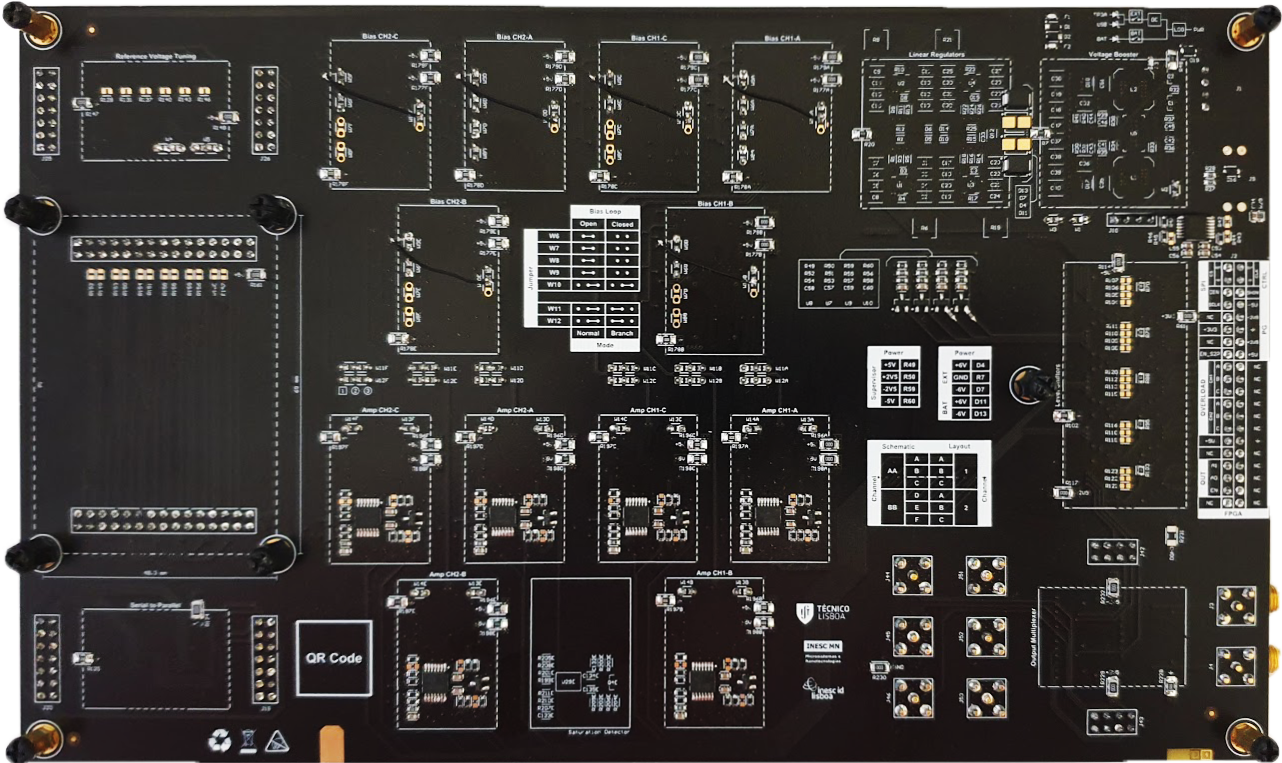
\includegraphics[width=\textwidth]{images/chapter_4/discussion_results/pcb_back.png}
        \caption{PCB back-view.}
        \label{figure:back-pcb}
    \end{subfigure}
    \caption{Cytometer platform version 3.0 PCB.}
    \label{figure:cyto-pcb}
\end{figure}

The resulting \ac{PCB} from this work is displayed in Figure \ref{figure:cyto-pcb}, illustrating its considerable size due to the absence of space constraints. However, there is potential for easy compaction by separating the modules into distinct \ac{PCB}s and integrating them together. This board represents the culmination of the \ac{3D} models showcased throughout this chapter. In addition to module design and layout considerations, the board design also prioritized the separation of analog and digital signals. A star grounding scheme was implemented, keeping the digital and analog grounds separate and connecting them in the power supply circuit. This design feature effectively minimizes noise and interference, ensuring the integrity and reliability of the signals. Given that digital signals are prone to generating noise and electrical disturbances due to their rapid transitions and high-frequency components, this separation is essential. The star grounding technique effectively reduces ground loop issues, crosstalk, and electromagnetic interference. The work conducted in this thesis also involved the soldering and debugging of the board, addressing some manageable issues that required hotfixes. Figure \ref{figure:front-pcb} provides a front view of the board, highlighting the key modules, while Figure \ref{figure:back-pcb} offers a back view, showcasing minor modules such as the saturation detect and power supervisors. It is important to note that all the newly featured modules were designed with contingency plans in case of module failure or malfunction, demonstrating a proactive approach to ensure system robustness and reliability.

% ----------------------------------------------------------------------------- Noise Measurements
\mytitle{Noise Measurements}

\noindent
\ac{MR} sensors are specifically designed to detect minute changes in magnetic fields by measuring variations in their resistance. These sensors generate extremely small electrical signals in response to magnetic field changes. However, due to the small amplitude of these signals, they are highly susceptible to the presence of noise. Despite their high sensitivity to magnetic fields, \ac{MR} sensors are also vulnerable to external noise sources. Real-world environments often expose \ac{MR} sensors to various forms of electromagnetic interference, including power lines, electromagnetic radiation, and nearby electronic devices. These interferences can introduce errors and distort the sensor signals, compromising the accuracy of the measurement results. To ensure reliable and precise measurements, it is of utmost importance that the noise introduced by the interface system is kept significantly lower than the inherent noise of the \ac{MR} sensors. By minimizing noise-induced fluctuations, the accuracy of magnetic field measurements can be preserved. Therefore, implementing an ultra-low noise interface is essential in order to mitigate the impact of noise and interference, allowing the \ac{MR} sensors to perform optimally and providing accurate detection of magnetic field changes.

For the \ac{SV} sensors used in this application, the two primary sources of noise are flicker noise (also known as pink noise or $\mathrm{1/f}$ noise) and thermal noise (also known as Johnson noise)\cite{freitas2007magnetoresistive}. In addition to the inherent noise of the sensors themselves ($e^2_{n_{sen}}$), the interface circuitry also contributes to the overall noise level. This includes the biasing architecture($e^2_{n_{bias}}$), sensor addressing ($e^2_{n_{addr}}$), amplification scheme ($e^2_{n_{amp}}$), and output multiplexing ($e^2_{n_{mux}}$). The noise introduced prior to the first amplification stage is particularly significant. As explained before, according to Friis' formula, the total noise figure of each stage is divided by the gain of all preceding stages. Since the first stage has the highest gain, the majority of the system's overall noise is attributed to this initial stage. Noise is characterized as an unwanted disturbance caused by random electrical fluctuations within a device. The total noise of the measurement can be quantified using Equation \ref{equation:total-noise}.
\begin{equation}
    e^2_{n_{total}} = e^2_{n_{sen}} + e^2_{n_{addr}} + e^2_{n_{bias}} + e^2_{n_{amp}} + e^2_{n_{mux}} \quad\left[\frac{V^2}{Hz}\right]
    \label{equation:total-noise}
\end{equation}

By carefully designing and optimizing the interface circuitry, it becomes possible to mitigate noise contributions and enhance the \ac{SNR}. This improvement in \ac{SNR} leads to enhanced accuracy and reliability of the measurements. To evaluate and quantify the overall noise, a Baseband Signal Analyzer was employed. The analysis involved conducting tests in three different scenarios: shorting the sensor terminal, using a resistance with known thermal noise, and utilizing a \ac{MR} sensor introducing both thermal and flicker noise. In the first scenario, only the noise from the amplification scheme and output multiplexing is considered, as the inputs of the differential amplifier are shorted. When a resistance is introduced, it incorporates the noise from the biasing, addressing, and thermal components. In the third scenario, the main difference observed should be the presence of a higher flicker noise. Additionally, the system's gain was measured using an Analog Discovery. The results of these measurements are depicted in the figure below:

\begin{figure}[!ht]
    \centering
    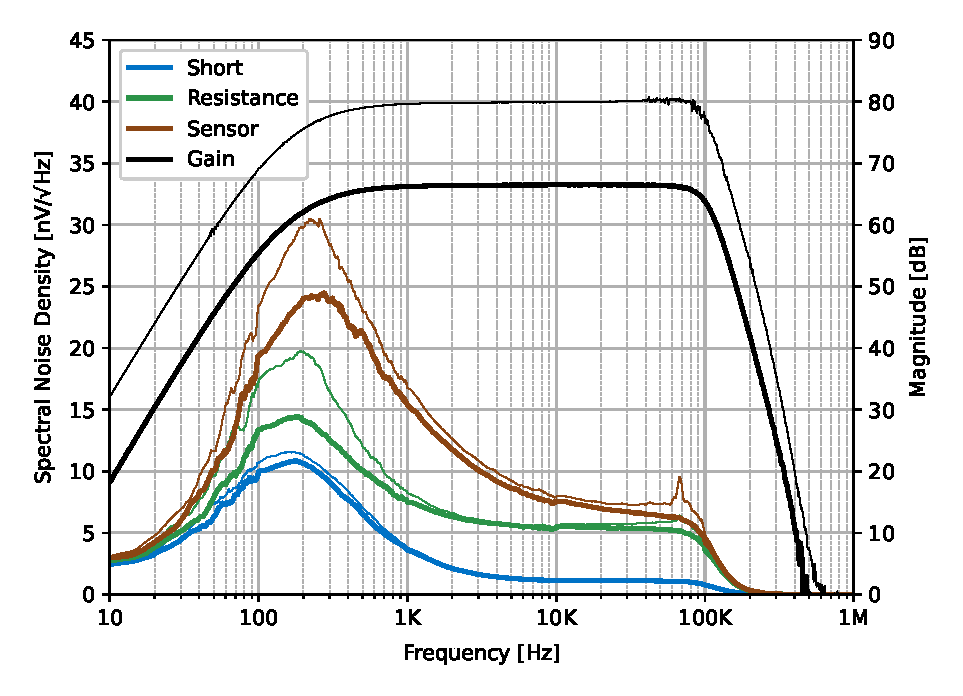
\includegraphics[width=.65\textwidth]{images/chapter_4/discussion_results/noise.eps}
    \caption{Noise measurements -- Comparison between the old platform and the one presented in this work.}
    \label{figure:noise}
\end{figure}

The measurements presented in Figure \ref{figure:noise} offer valuable insights into the noise characteristics and gain of the system. The graph displays the measurements for both platforms, with the thicker line representing the interface developed in this work and the thinner line representing the previous interface developed by Eng. Ruben Afonso. Interestingly, despite the incorporation of additional features such as sensor addressing and output multiplexing in this version, the noise was successfully reduced compared to the previous version. This outcome is noteworthy, as the introduction of these features could potentially introduce additional noise. Thus, it was expected to observe similar or higher levels of noise in this version. However, the measurements demonstrate a significant improvement in noise reduction, emphasizing the effectiveness of the design optimizations implemented in this work. This result can be attributed to the biasing architecture, as evidenced by the comparable noise levels observed when the terminals are shorted. The noise introduced by the sensors addressing is minimal and primarily influenced by the thermal noise of the Ron resistances of the multiplexers. Given that the biasing topology remains similar between the two platforms, the primary difference lies in the reference voltage module. Specifically, the implementation of an XFET reference in the new platform has proven advantageous, offering superior noise performance compared to the previous use of buried Zener references. This successful implementation has effectively reduced the overall noise, even with the addition of additional features. As expected, the flicker noise in the scenario involving the sensor was higher, while the baseline noise should have remained the same in both the resistance and sensor scenarios. However, an incongruous result was obtained where the baseline noise was also higher in the sensor scenario. This unexpected outcome can be attributed to the mismatch in resistance values used for the test. Specifically, the resistance employed had a value of $\mathrm{1~k\Omega}$, whereas the sensor had a nominal value of $\mathrm{1.2~k\Omega}$. The difference in gain between the two interfaces can be attributed to the implementation of the output multiplexer circuit. This circuit incorporates voltage dividers to ensure that the output signal adheres to the $\mathrm{2~V}$ peak-to-peak limitation set by the \ac{FPGA} \ac{ADC}s. By using voltage dividers, the signal is properly scaled to match the input range of the \ac{ADC}s, thus accounting for the disparity in gain observed between the interfaces.

In conclusion, the implemented strategies and circuitry optimizations successfully reduced the noise introduced by the system. Through careful design, noise-reducing techniques, and advanced noise management, the \ac{SNR} was significantly improved. These efforts resulted in a more robust and reliable interface, enabling accurate measurements in the presence of external noise sources.
% ----------------------------------------------------------------------------- Noise Measurements

% ----------------------------------------------------------------------------- Magnetic Field Measurements
\mytitle{Magnetic Field Measurements}

\noindent
In order to conduct thorough testing of the cytometer platform and fulfill its intended purpose, the inclusion of \ac{MR} sensors was crucial. The platform relies on the presence of a magnetic field to detect and measure changes in the \ac{MR} sensor resistance. Therefore, it was necessary to generate a magnetic field to stimulate the sensors and evaluate their performance within the cytometer system.

To generate the required magnetic field for the testing of the cytometer platform, a system developed by Eng. Fabian Näf was utilized. This system consists of two coils and a driver power op-amp. The driver power op-amp serves the purpose of amplifying a known sinusoidal waveform, which is then injected into the coils. As per the Biot-Savart law, the current flowing through the coils creates a magnetic field. The configuration of the two coils is crucial to achieve the desired magnetic field characteristics. They are positioned with a specific distance between them in order to create a nearly uniform magnetic field. This specific configuration is commonly referred to as a Helmholtz coil pair, providing a consistent and controlled environment for the \ac{MR} sensors. By utilizing Fabian's system, comprised of the coils and the driver power op-amp, it was possible to generate the necessary magnetic field to stimulate the \ac{MR} sensors. This allowed for accurate and reliable testing of the platform's performance and validation of its intended functionality.

One of the performance tests that can be conducted using Fabian's system is the evaluation of harmonic distortion in the cytometer platform. Harmonics are additional frequencies that were not present in the original signal and alter the waveform shape, a common occurrence in electronic systems and circuits. However, in many cases, harmonics are undesirable and can be considered as noise or distortion. When harmonics are present in a system, they have the potential to interfere with the desired signal and introduce distortion or degradation in signal quality. This can lead to inaccurate signal representation or the presence of unwanted artifacts. Therefore, it becomes crucial to manage harmonic distortion by attenuating these unwanted harmonic components. By ensuring appropriate harmonic attenuation, signal integrity can be maintained, and distortion can be minimized. This is particularly important in the context of the cytometer platform, a sensitivity application, that requires an accurate and reliable signal detection and analysis.

\begin{figure}[!ht]
    \centering
    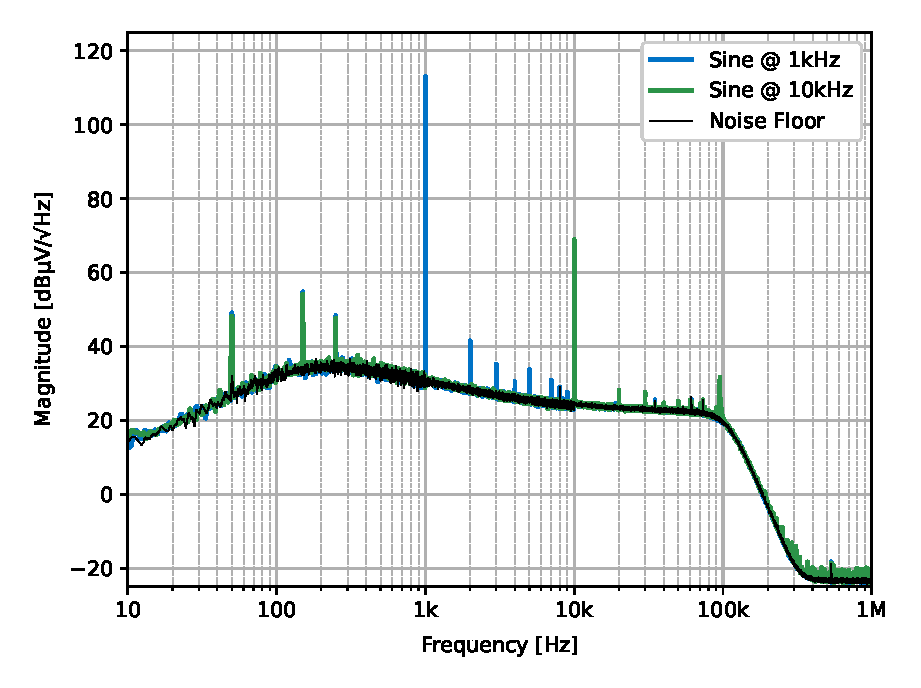
\includegraphics[width=.65\textwidth]{images/chapter_4/discussion_results/harmonics.eps}
    \caption{Magnetic field measurements.}
    \label{figure:harmonics}
\end{figure}

Figure \ref{figure:harmonics} depicts the results of the harmonic performance analysis of the system. The test involved two experiments, each utilizing a magnetic field with different frequencies. The blue trace represents the $\mathrm{1~kHz}$ frequency, while the green trace represents the $\mathrm{10~kHz}$ frequency. In the blue trace, it is evident that the system exhibits an impressive attenuation of approximately $\mathrm{70~dB}$ between the 2\textsuperscript{nd} harmonic and the 1\textsuperscript{st} harmonic at a fundamental frequency of $\mathrm{1~kHz}$. This level of attenuation is especially desirable in this sensitive application, as it ensures precise signal reproduction and minimizes distortion. Achieving such a high level of attenuation is crucial for maintaining signal integrity and fidelity. The attenuation observed in the green trace is lower than the blue trace, but this is primarily attributed to the frequency response characteristics of the Helmholtz coil driver rather than the platform itself. The coil driver operates based on voltage, and the voltage value was adjusted to maximize the dynamic range of the system, reaching a peak-to-peak voltage of $\mathrm{2~V}$. However, it is important to note that the magnitude of the magnetic field is determined by the current flowing through the coil, not the voltage. As the frequency increases, the reactance of the coil, also known as the "coil resistance," begins to rise. The used Helmholtz coil has an inductance of $\mathrm{538~\mu H}$, which results in a reactance of $\mathrm{3.38~\Omega}$ at $\mathrm{1~kHz}$ and $\mathrm{33.8\Omega}$ at $\mathrm{10~kHz}$. Since the voltage remains constant, the current flowing through the coil is reduced to compensate for the increasing resistance. Consequently, the magnitude of the magnetic field produced by the coil decreases at higher frequencies. The observed decrease in the magnetic field magnitude at higher frequencies is a consequence of the interplay between the coil resistance, voltage, and current. 

The harmonic performance results demonstrate the system's capability to effectively suppress undesired harmonic components and preserve the integrity of the desired signal. These findings highlight the system's suitability for applications requiring accurate and distortion-free signal processing.

% ----------------------------------------------------------------------------- Magnetic Field Measurements
% ############################################################################# Discussion and Results

\clearpage
\thispagestyle{empty}
\cleardoublepage